%%%%%%%%%%%%%%%%%%%%%%%%%%%%
% Master's Thesis          %	    										
% Fabian Burth, 2022-08-01 %
%%%%%%%%%%%%%%%%%%%%%%%%%%%%	

\npchapter{System Design}
This section describes the design of the \textit{Security and Compliance Data Lake}. It covers the conception of the data model, the selection of a database and the design of the API. Thereby, it especially discusses alternatives and focuses on giving detailed information about the ideas and motives that led to specific design decisions.

\section{Requirements}
Before actually going into the details of the systems design, the requirements have to be specified, since they are at the core of every design decision.  

\subsection{Functional Requirements}
The below table \ref{Tab:Requirements} provides a condensed list of the functional requirements for the Security and Compliance Data Lake. Thereby, every requirement is described by a short and precise but abstract statement of what functionality the system must have and an additional explanation which also includes an example. Additionally, there is a column categorizing the requirements as priority 1 or 2.\par 
Priority 1 is functionality deemed necessary for a central metadata store which should solve the limitations and problems identified in the previous chapters. Furthermore, priority 1 functionality is usually functionality that has to be considered in the design process and otherwise cannot be easily added without foundational remodeling.\par
Priority 2 functionality describes convenience features which are less urgent and may easily be added later on.
\begin{xltabular}{\linewidth}{|l|X|l|}
	\hline \hline \rowcolor{lightgray} \multicolumn{3}{ |l| } {\cellcolor{lightgray}{\textbf{Requirements}}}
	\\ \hline \rowcolor{lightgray}\textbf{Ref.\#} & \textbf{Functionality} & \textbf{Prio.}
	\\ \hline
	\endfirsthead
	
	\hline \hline \rowcolor{lightgray}\multicolumn{3}{|l|}{\cellcolor{lightgray}{\textbf{Requirements}}} \\ \hline \rowcolor{lightgray} \textbf{Ref.\#} & \textbf{Functionality} & \textbf{Prio.}\\ \hline
	\endhead
	
	\hline \multicolumn{3}{|r|}{{Continued on next page}} \\ \hline
	\endfoot
	
	\hline \caption{Requirements} \label{tab:Requirements}
	\endlastfoot
	
	R.1 & The SCDL shall be able to consume and store metadata from multiple different data sources.\newline\newline
	The SCDL shall be able to work with any kind of metadata about software components.	Therefore, it has to be able to handle multiple different scanning tools as well as other kinds of data sources like build tools. As an example, it may have to consume data from BDBA, Mend but also Jenkins. Thus, it has to be considered that besides vulnerabilities and licenses, a variety of other metadata types may need to be added in the future. & 1\\
	\hline
	R.2 & The SCDL shall store the metadata from different data sources without aggregation\footnotemark{}.\newline\newline
	Different tools that generally serve the same purpose may provide similar information. As an example, BDBA and Mend are both SCA tools and therefore provide overlapping results. To ensure that no data is lost, this information shall not be combined and aggregated before storing.
	\footnotetext{\textit{aggregation} in this context means to merge the data about a package of e.g. a BDBA scan and a Mend scan to a single package entity instance} & 1\\
	\hline
	R.3 & The SCDL shall provide the metadata from different data sources with aggregation\footnotemark[\value{footnote}].\newline\newline
	As mentioned before, to ensure no data is lost, the data from different data sources shall be stored without aggregation. Anyway, to be consumed by a user, this data shall be aggregated. As an example, when querying all packages contained in a specific resource, the result returned by the SCDL shall not contain the same package twice in different representations, if it was identified by BDBA and by Mend. Instead, it shall contain an aggregated representation of the package. Thus, some kind of aggregation layer is needed which provides transparency regarding the data sources. & 1\\
	\hline
	R.4 & The SCDL shall provide a level of aggregation\footnotemark{} to group sources and resources.\newline\newline
	\footnotetext{\textit{aggregation} in this context refers to the "whole/part" semantic of the word \cite{UML}. Thus, since resources and sources are comprised of packages, they are both aggregations of packages. On a model level, the same applies for the relationships between packages and vulnerabilities or licenses as well as between entire deployments and the deployed resources.}
	As pointed out before, one problem also with SBOMs is the disconnection of the artifact metadata and the deployment information. To bridge this gap, an additional aggregation level for grouping artifacts is necessary. As an example, this additional aggregation level shall enable to group all resources contained in a specific deployment. & 1\\
	\hline
	R.5 & The SCDL shall enable users to query the metadata on different levels of aggregation\footnotemark[\value{footnote}]\newline\newline
	As an example, a user shall be able to query for all vulnerabilities in a specific resource, thus query on the aggregate level of resources. But a user shall also be able to query for all vulnerabilities in an entire specific deployment, thus querying on the aggregate level of deployments (querying on this level of aggregation enables to answer where Log4J is deployed). & 1\\
	\hline
	R.6 & The SCDL shall enable users to perform assessments.\newline\newline
	The relevance of specific pieces of information such as vulnerabilities or licenses depends on the usage context. As an example, while the internal usage of an altered OSS with a copyleft license is lawful, the distribution is not. Therefore, a possibility has to be provided to assess such pieces of information in the context of their occurrence. & 2\\
	\hline
	R.7 & The SCDL shall provide common data aggregation and filter functions for the queries.\newline\newline
	As an example, a user shall be able to filter for the vulnerability with the highest CVSS within a resource or shall be able to get the count of vulnerabilities within a resource. & 2\\
	\hline
	R.8 & The SCDL shall enable users to query the metadata in the common SBOM formats.\newline\newline
	In order to be able to fulfill governmental requirements of the executive order mentioned in the Software Bill of Materials section, the SCDL has to provide a way to to query the metadata in the common SBOM formats. As an example, a user shall be able to query the SPDX document for a specific resource. & 2\\
\end{xltabular}

So, by fulfilling this functional requirements, the Security and Compliance Data Lake may actually serve as a central application for storing and querying software metadata. Thereby, solving the problem of metadata being distributed throughout the development life cycle and bridging the gap between artifact metadata and deployment information.

\subsection{Non-functional Requirements} \label{sec:Non-functional Requirements}
Since this shall be a prototypical implementation, there is a strong focus on fulfilling the functional requirements. Thus, no concrete limits regarding performance or scalability such as a maximum response time of 5 seconds or support for up to 1000 concurrent users are set here. Considering the novelty of the topic, there is very few reference data and therefore, such specifications would be premature. However, for a central metadata store which may prospectively power dashboard web applications for monitoring purposes, scalability and performance definitely have to be considered in design decisions already.

\section{Data Model}
The basic entities relevant in the software supply chain are artifacts, thus sources and resources, and the packages comprising these artifacts. The definition of sources and resources is still the same as introduced in the previous chapter. Resources are capable of doing something and are usually executables or OCI Images. Sources are the code the resources are built from. Compliance scanners usually scan entire source code repositories or binaries. Through different methodologies, these tools detect the packages contained in these scanned artifacts on a best effort basis. In the context of this work, a package is defined as functional unit contained in artifacts, whereby it is usually a collection of files forming a library which is imported in the source code. By subsequently matching these packages against different databases such as the NVD, introduced in section \ref{sec:Vulnerability Management} "Vulnerability Management", known vulnerabilities and licenses are identified. To give a better idea of these results, figure \ref{fig:bdbaResult} in the appendix shows a snippet returned from the API of BDBA. The results on their own are useful already and provide interesting data about the above mentioned entities. But it is still loose metadata that lacks context information such as which deployments contain the corresponding entities. Therefore, an additional entity type to conduct further grouping is required. The OCM already introduced such an entity type, the component.\par
To conclude this, from a high level perspective, the important entities are \emph{components}, \emph{sources}, \emph{resources}, \emph{packages} and the information attached to these entities such as vulnerabilities and licenses. To generalize this and abstract away from specific data sources, the entity type representing these types of metadata is called \emph{info snippet}. So these entity types are the basic building blocks for the data model. From here on, it is getting rather complex and abstract. To still keep the explanations tangible, below figure \ref{fig:DataModel} already shows an \emph{entity-relationship model (ERM)} describing the final and universal data model. This may be used as a reference point throughout the following paragraphs, discussing the design decisions leading up to the specific entities, relationships and cardinalities.

\begin{figure}[H]
	\centering
	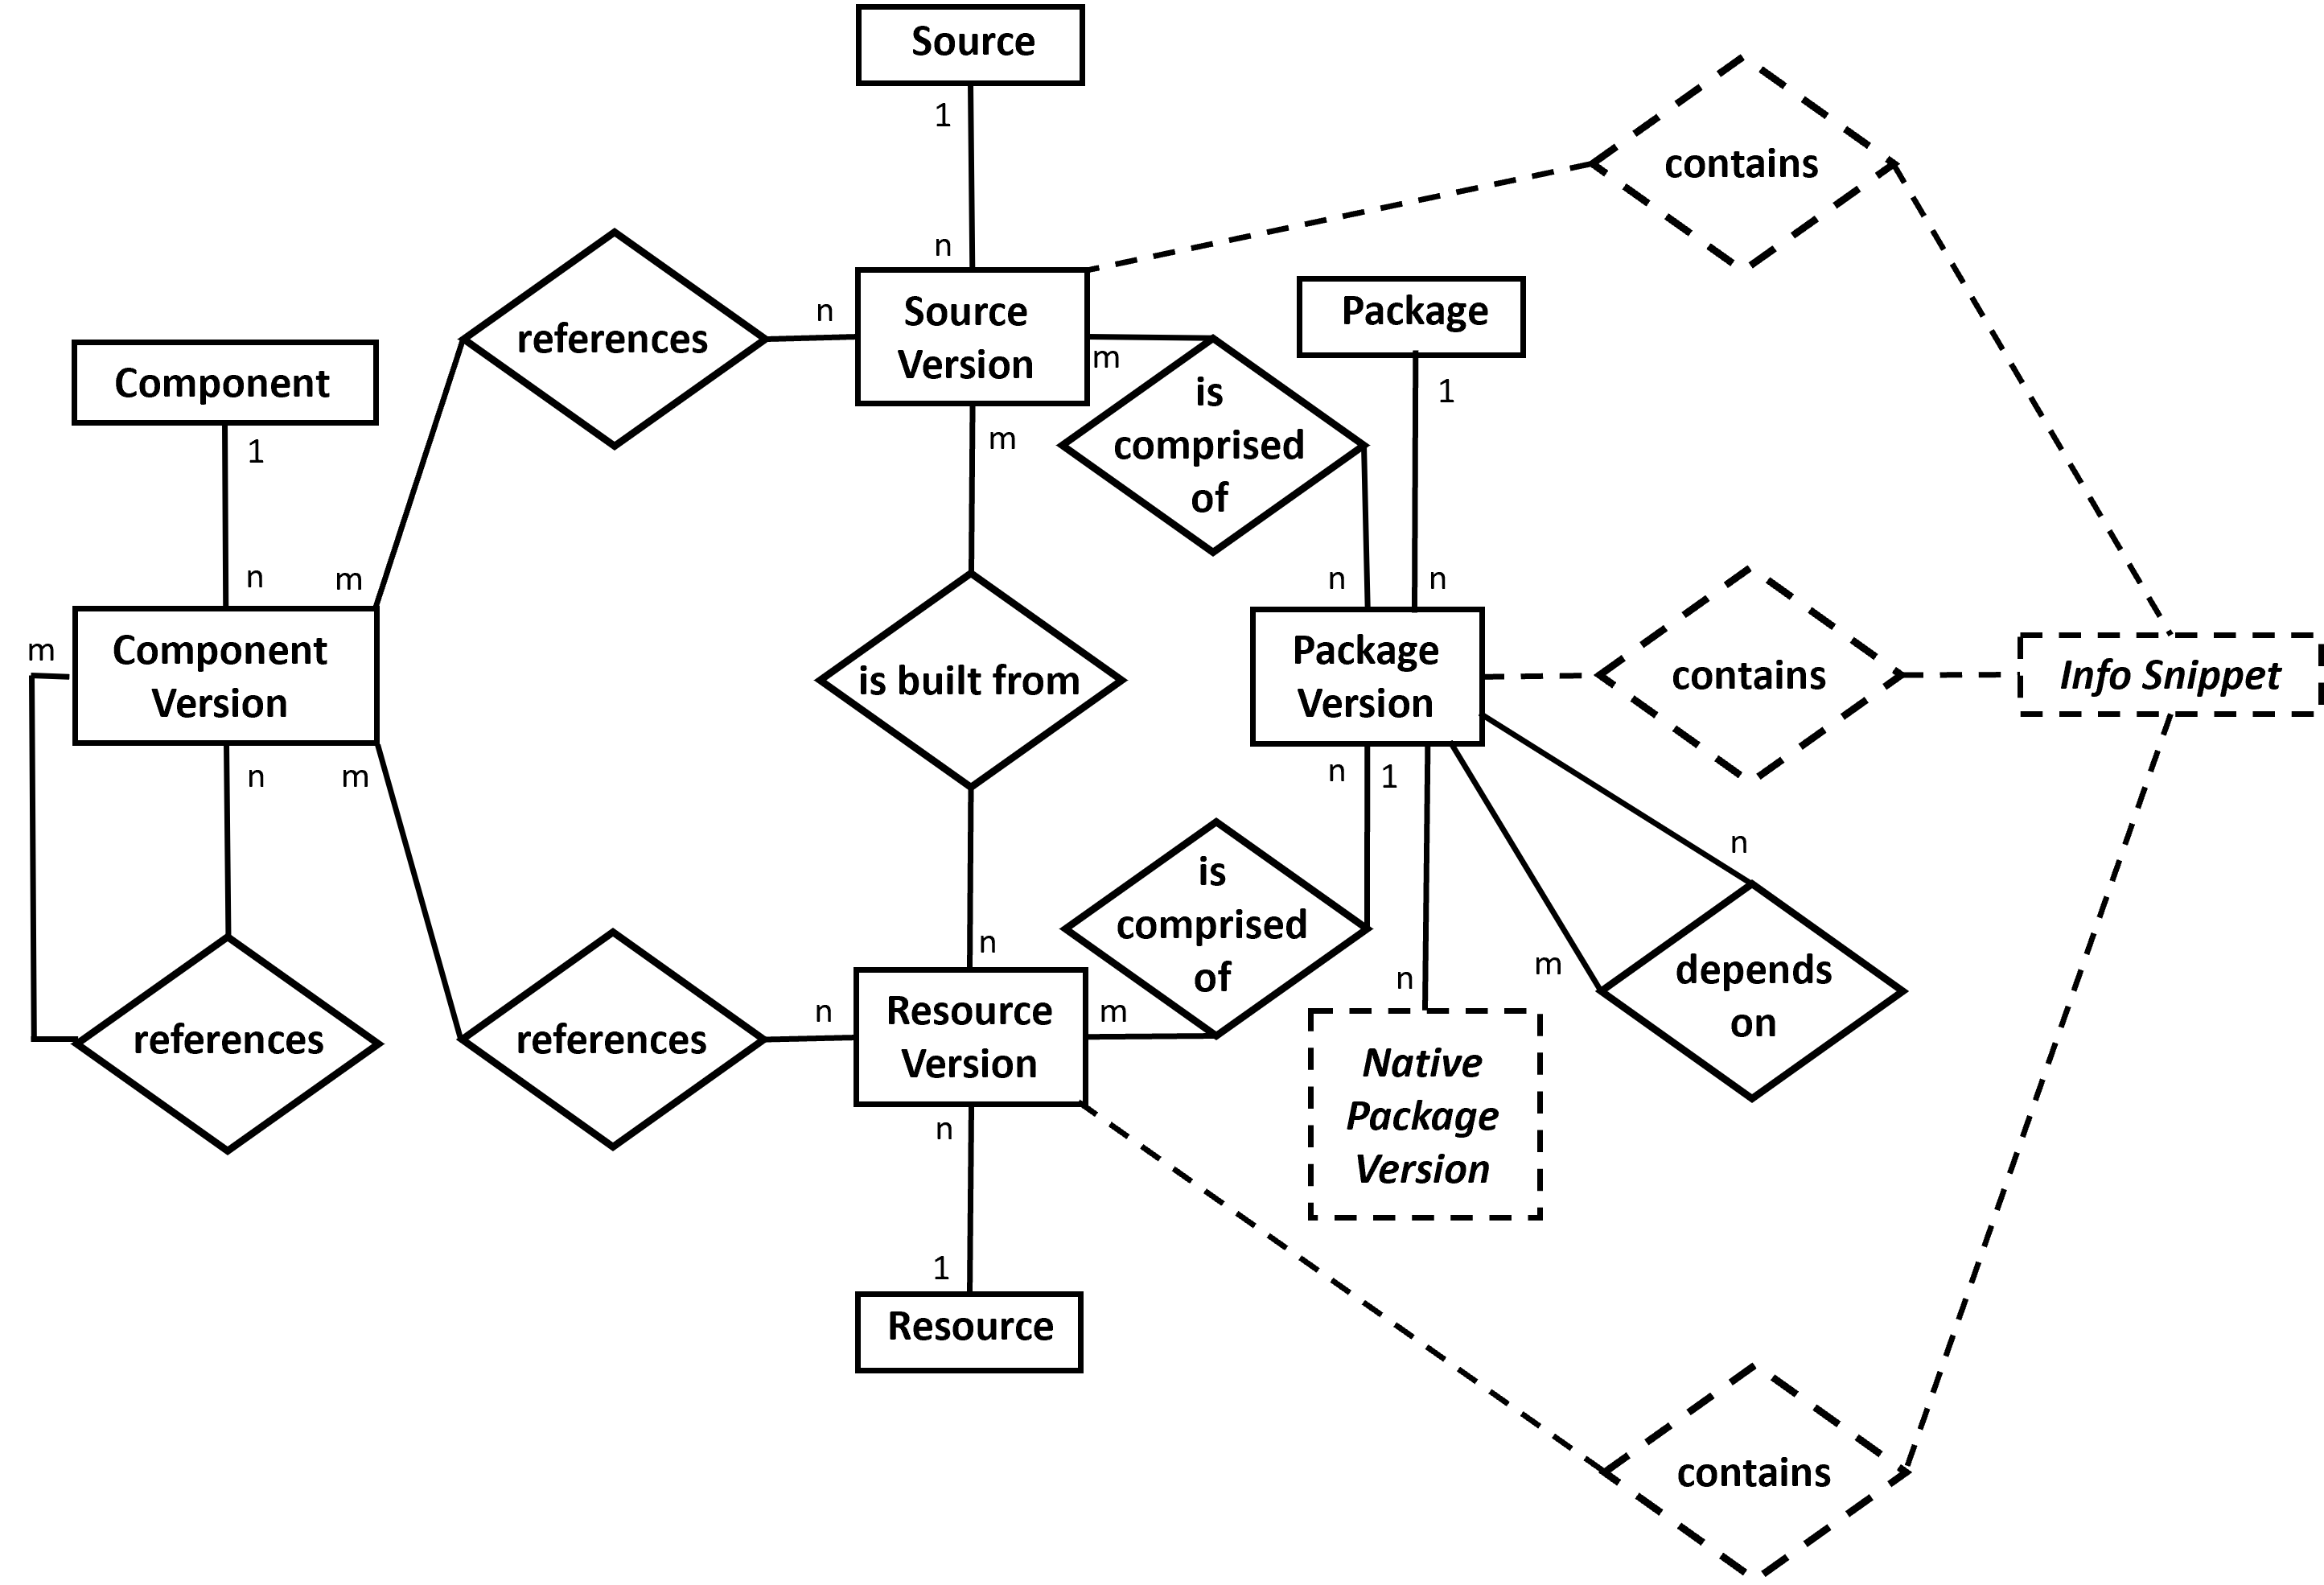
\includegraphics[scale=0.65]{datamodel}
	\caption[Data Model]{Data Model \source{Own Representation}}
	\label{fig:DataModel}
\end{figure} 

Even though the motivation behind every element may not be obvious immediately, the model as a whole should feel quite familiar and intuitive by now. An important notice at this point, the data model is inspired by the OCM. As mentioned above, especially the entity type \emph{component} is lend from the OCM. Since this thesis is written within SAP Gardener, a seamless integration of the this Security and Compliance Data Lake such as described in the previous chapter is of course also a requirement, even though it is not explicit listed. But still, the Security and Compliance Data Lake is designed independent of the OCM. Thus, in theory it is entirely possible to use a different kind of component model. As an example, if one is able to express the concept of \emph{components} and \emph{artifacts} with the means of the SPDX standard, one could use SPDX instead of OCM to provide this structural information. Or, since SPDX is not optimal for this purpose, one could create and use an own component model, as long as it has the means to express \emph{components} and \emph{artifacts} (There is generally no necessity to distinct between \emph{sources} and \emph{resources}. \emph{Sources} could be treated as \emph{resources}, at the only cost of losing the connecting "is built from"-information between the two entities.).

\subsection{Universal Data Model}
Contrary to common ERMs, the one in figure \ref{fig:DataModel} does not have any properties. There are two major reasons for this. Firstly, the just mentioned independence of a specific component model would hardly be possible if the data model would define fixed predefined properties for each entity type. Secondly, the different scanning tools provide a wide range of information about packages and other data sources but scanning tools may also be added. It is therefore practically impossible to foresee what properties may be needed. Besides, these may vary depending on the user of the Security and Compliance Data Lake.\par
Another special feature of above ERM are the entity types and relationships illustrated with dash lines. These represent classes of entity types and relationships. Since the whole set of data sources cannot be known upfront, the whole set of potentially required \emph{Info Snippets} cannot as well. As already mentioned in several examples before, when adding a build tool as data source, an entity type \emph{Build Information} may be needed. Also, the relationships of different \emph{Info Snippet} entity types may vary. While a \emph{Vulnerability} and a \emph{License} is usually \emph{contained} in multiple \emph{Package Versions} leading to a (n:m)-relationship, a \emph{Build Information} is usually associated to one \emph{Resource Version} leading to a (1:n)-relationship. But generally, \emph{Info Snippets} could be associated to any other entity type in the data model with any cardinality. This kind of flexibility is necessary to enable R.1 (consume and store metadata from multiple different data sources). The \emph{Native Package Version} correspondingly illustrates the representation of a package, native to a concrete data source. Thus, instances of \emph{Native Package Versions} may be \emph{BDBA Package}, \emph{Mend Package} or even \emph{Jenkins Package}. So if all three data sources provide information about the exact same \emph{Package Version}, each representation may be stored without a need to merge their properties before storing. Thereby, this enables R.2 (store metadata from different data sources without aggregation). Then, a set of properties commonly provided by all of the data sources may be aggregated on \emph{Package Version} level, thereby also enabling R.5 (provide the metadata from different data sources with aggregation). So, all these \emph{Native Package Versions} representing the exact same package are related to the same \emph{Package Version} on the model level. As the different data sources may use different identifiers for the packages, the merging process cannot be triggered automatically. Hence, until a human defines that the \emph{BDBA Package}, the \emph{Mend Package} and the \emph{Jenkins Package} are actually representations of the same package, no merging is done and each is related to a different \emph{Package Version}.\\\par
So after explaining the special features of above ERM, the common entity types and relationships may be discussed. The basic entity type \emph{component} is broken down into two distinct entity types, \emph{Component} and \emph{Component Version}. As immediately noticeable, this distinction is done for each of the basic entity types. \emph{Component} is a purely abstract entity type. It merely groups all the versions of the same component together. Thereby, the \emph{Component} may provide information about the semantics of this grouping such as whether this \emph{Component} describes a specific deployment or whether it describes all software used by a department. Thus, information that is identical for all versions of this component and would have to be stored redundantly for each \emph{Component Version} otherwise. Naturally, there are multiple \emph{Component Versions} of each \emph{Component}. Therefore, the (1:n)-cardinality here is self-explaining.\par 
As established by the previously described grouping semantic of \emph{components}, a \emph{Component Version} may reference multiple other \emph{Component Versions}. For example, a \emph{Component Version} describing a specific version of a deployment may reference multiple other \emph{Component Versions} such as \emph{Component Versions} describing specific versions of a web server, a service and a database. Reciprocal, a \emph{Component Version} may of course be referenced by multiple \emph{Component Versions}. For example, a \emph{Component Version} describing a web server may be referenced by several \emph{Component Versions} describing different versions of the same deployment or entirely different deployments. Thus, this is a recursive (n:m)-relationship. There may also be a need to store additional occurrence specific metadata as properties of the \emph{references}. Considering the above example, such occurrence specific metadata may provide information about the usage of the web server within the deployment, hence whether it is used as a HTTP server or as a load balancer. Together, these model elements fulfill requirement R.4 (provide an aggregation level to group sources and resources).\par
Furthermore, a \emph{Component Version} may also reference multiple \emph{Source Versions} and \emph{Resource Versions}. As an example, the \emph{Resource Versions} comprising the web server and the \emph{Source Versions} from which the respective \emph{Resource Versions} were built. As before, with the recursive relationship of \emph{Component Versions}, the \emph{Source Versions} and \emph{Resource Versions} may of course also be referenced by multiple \emph{Component Versions}, resulting in a (n:m)-relationship. Again, there may be a need to store additional occurrence specific metadata as properties of the \emph{references}. Specifically, these \emph{references} may be used to store \emph{triage} information. As this \emph{reference} describes the usage context of the \emph{Artifact}, one may for example decide whether a copyleft license is or is not acceptable here. The relationship between \emph{Source} and \emph{Source Version} as well as between \emph{Resource} and \emph{Resource Version} is similar to the relationship between \emph{Component} and \emph{Component Versions}. But the abstract \emph{Source} and \emph{Resource} entity types actually do have a concrete purpose but only preventing redundant storage of certain properties. In this case, these abstract entities may have properties to store \emph{triage policies}. As an example, one may store that a specific vulnerability may be ignored for the usage of \emph{Resource Versions} v1.0.0 to v1.2.3 of a respective \emph{Resource} within \emph{Component Versions} v1.4.2 to v1.4.12 of a specific \emph{Component}. The \emph{references} and the abstract \emph{Source} and \emph{Resource} entities thereby enable the fulfillment of requirement R.6 (enable users to perform assessments).\par 
\emph{Resource Versions} may also reference the \emph{Source Versions} they are built from. A \emph{Resource Version} may be built from multiple \emph{Source Versions} and a \emph{Source Version} may be used to build multiple \emph{Resource Versions}. This also results in a (n:m)-relationship.\par
Since \emph{Artifacts} are comprised of \emph{Package Versions} and the same \emph{Package Version} may occur in multiple \emph{Artifacts}, both \emph{Source Version} as well as \emph{Resource Version} have a (n:m)-relationship to \emph{Package Version}. Again, there may be a need to store additional occurrence specific metadata as properties of the \emph{is comprised of} relationship.\par
The relationship between \emph{Package} and \emph{Package Version} is again similar to the relationship between \emph{Component} and \emph{Component Versions}. But as already explained \emph{packages} are broken down even further into three different entity types and thereby three aggregate levels. Since several data sources may provide different representations, thus different \emph{Native Package Versions}, of the same \emph{Package Version}, the cardinality of this relationship is (1:n). \emph{Package Versions} frequently \emph{depend on} other \emph{Package Versions} and so on. This may lead to quite long chains of dependencies. This has to be kept in mind as these transitive dependencies are also relevant when trying to answer the question, whether a certain \emph{Artifact} or \emph{Component} contains a specific \emph{Package} such as Log4J, and its corresponding vulnerabilities.\par
Finally there is the \emph{Info Snippet} class of entity types. As explained above, different \emph{Info Snippet} entity types may have relationships to different entity types with different cardinalities.

\subsection{Insights into the Development Process}
At this point, some insight into the development process may be beneficial to understand this design decisions. The scope of this central data store was initially much narrower. The first PoC was actually strictly bound to the OCM. Therefore, the data model predefined the properties of \emph{component} and \emph{artifact} entity types. As it was bound to the OCM, there was no issue in doing so. But the data model also predefined the properties of the \emph{package} entity types. In fact, the third aggregate level for \emph{packages}, \emph{Native Package Version} did not exist at all. Instead, the \emph{Package Version} entity type had a set of properties that was hoped to be common and harmonizable throughout all prospective data sources. At this time, the application was also tailored to only having scanning tools as data sources. Therefore, to define this set of properties, the API documentations of different scanning tools were analyzed for the common and most important properties, especially the ones of BDBA and Mend \cite{MendAPI}. Additionally, to get a better understanding, both scanners were used on some artifacts to get some sample data. Then, the provided attributes were narrowed down and some interviews with developers were conducted. A huge effort was made here, as this was such an important decision. Also, instead of having the \emph{Info Snippet} class of entity types, there was only a \emph{Vulnerability} and a \emph{License} entity type whose set of properties was defined in the same process. Besides the fact that there was already a substantial amount of disagreement between different developers which properties were actually required, by the time the PoC was finished, several new use cases were discovered that required additional properties and even entire additional entities to provide other information than about vulnerabilities or licenses.\par
This led to a change in perspective, interpreting the task of defining the right entity types with the right properties rather as a task to make the entire application extensible regarding the respective entity types and properties. But this flexibility and extensibility comes at the cost of a highly increased overall complexity. Apart from remodeling the data model, it also required a completely new architecture and completely different implementation. Thus, only after that, the scope widened drastically, also allowing other component models. Consequently, as a kind of disclaimer, the design process presented here is not exactly as chronological as it may initially seem, since it hides a complete development iteration leading up to the final concepts.

\subsection{Application of the Data Model} \label{sec:Application of the Data Model}
Although a great effort was made to make the data model as tangible as possible, it may still be hard to grasp due to its abstract nature, omitting properties and introducing classes of entity types. Therefore, this section discusses how this data model could be applied. As reference component model, the OCM is used and as reference data sources, only BDBA is used. This thereby also reveals a problem that has to be faced when applying this data model to a real world use case. The figure \ref{fig:RefDataModel} below shows the corresponding data model instance.\par

\begin{figure}[H]
	\centering
	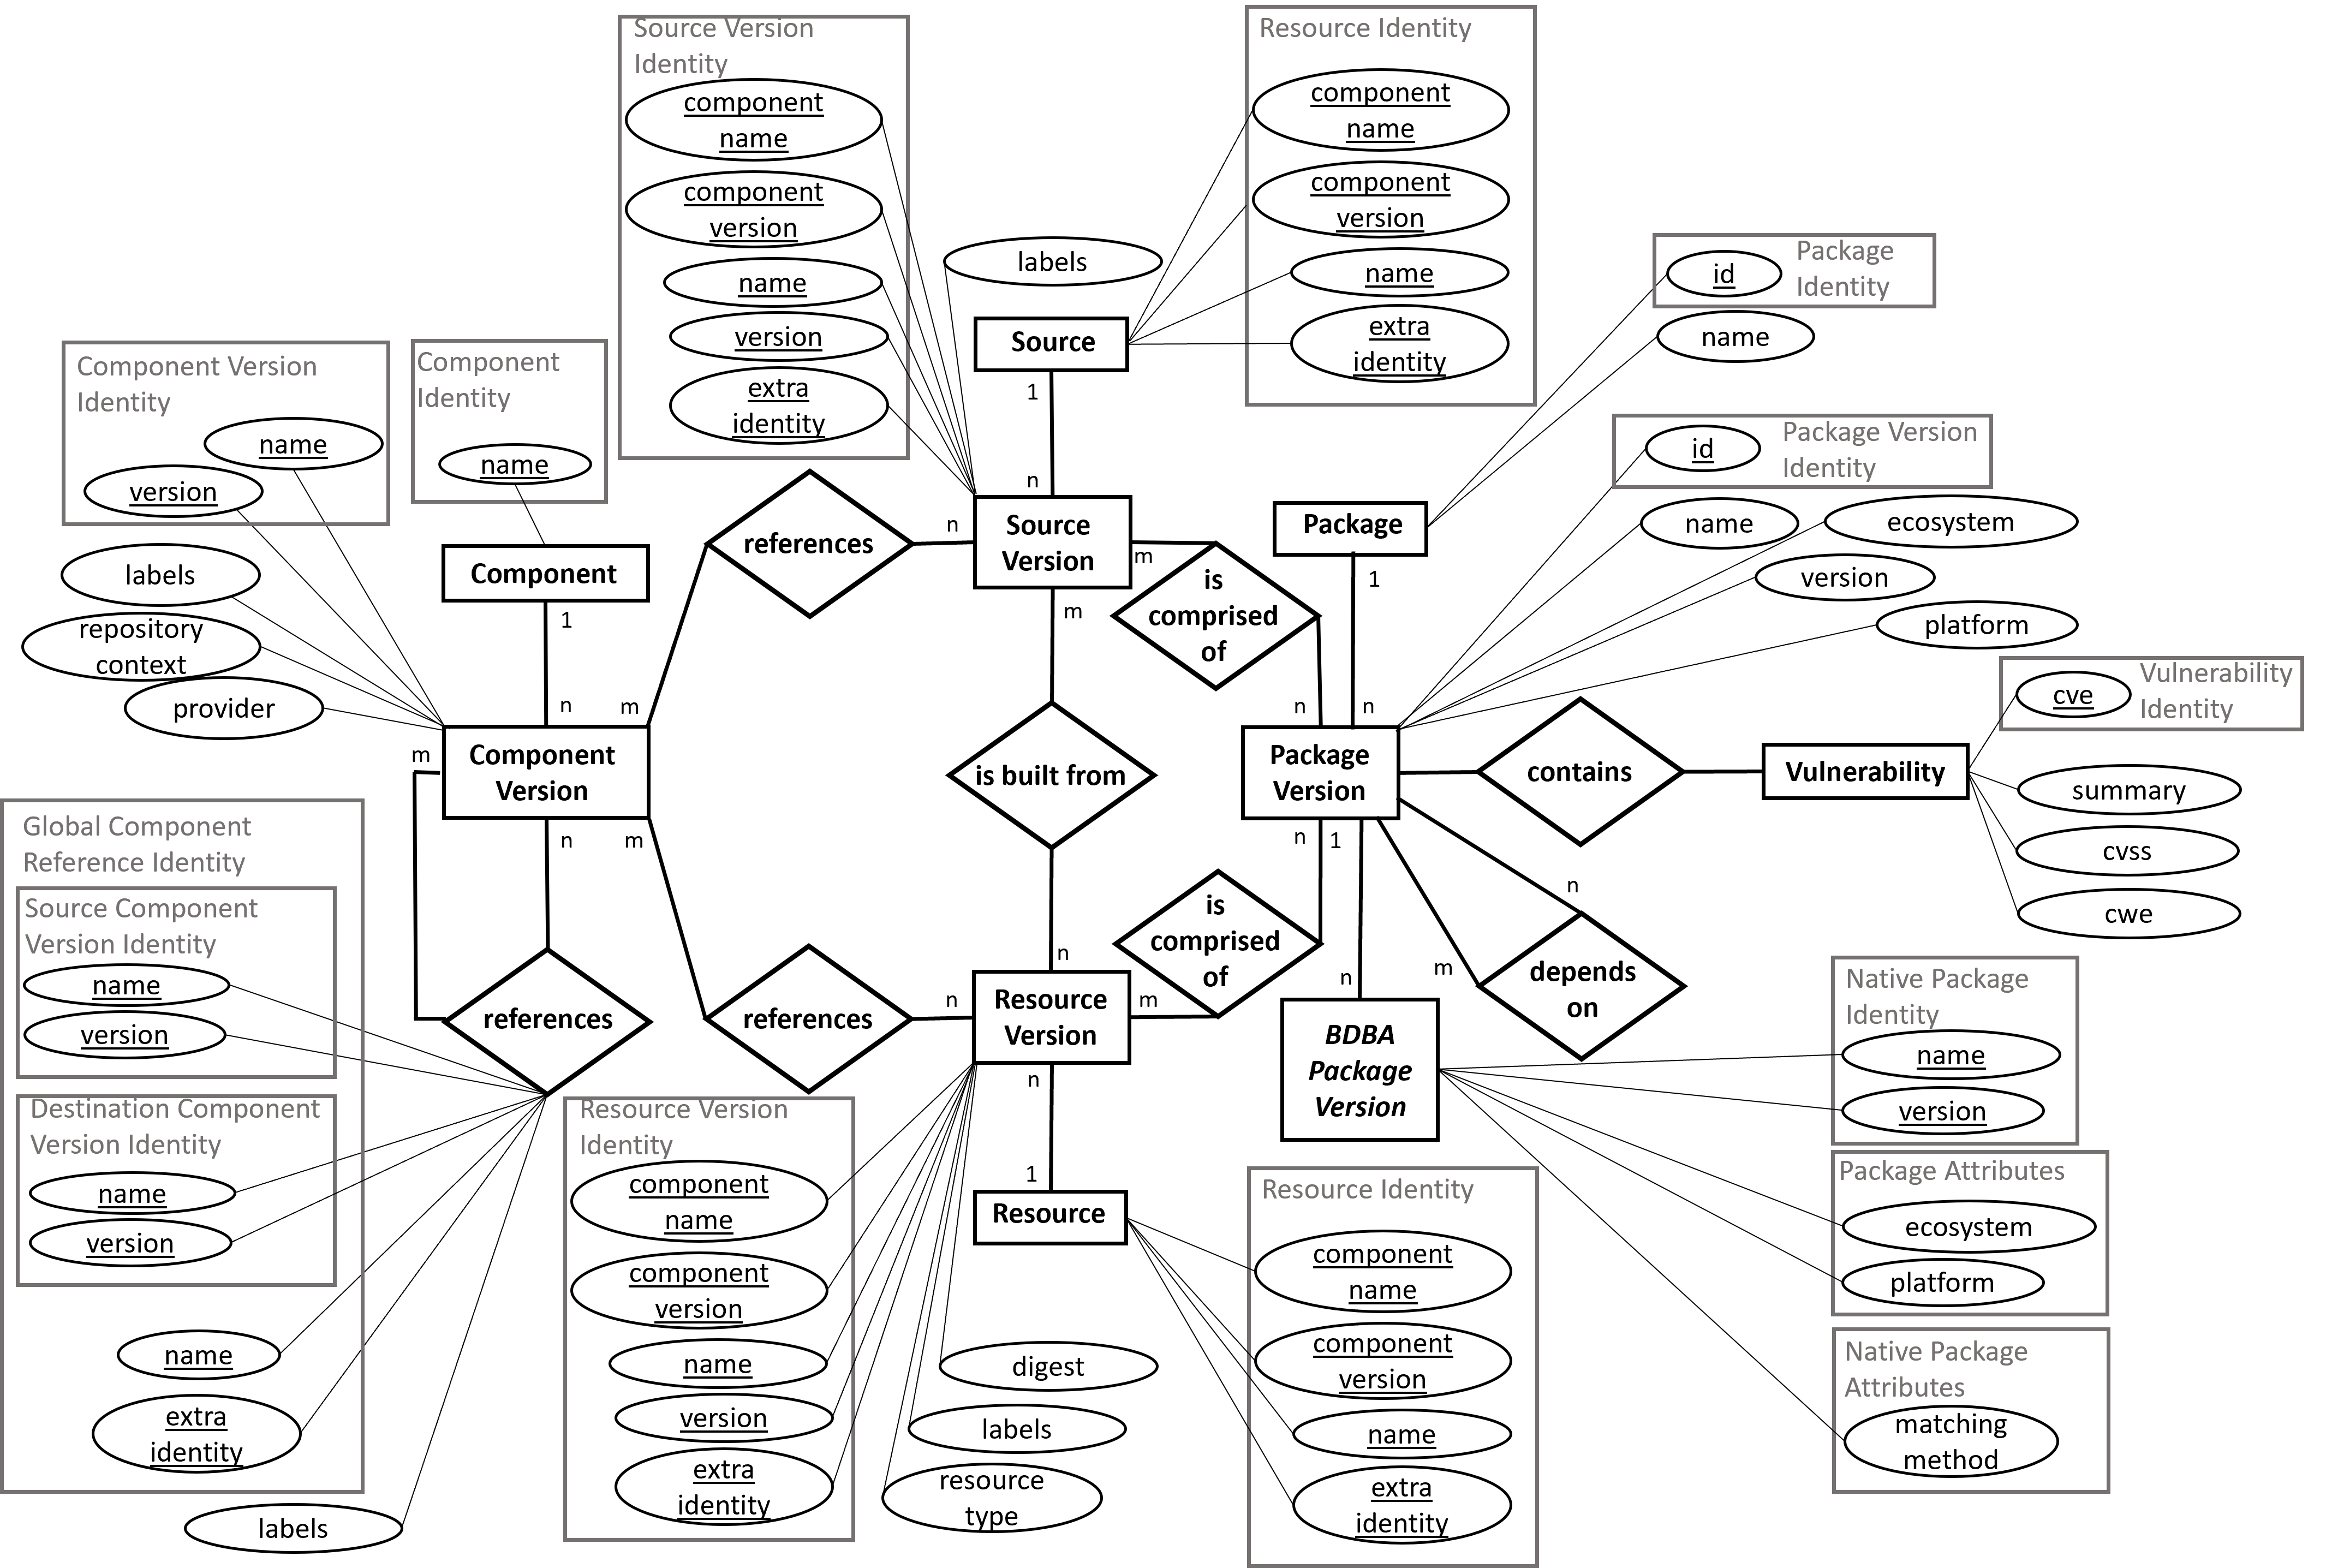
\includegraphics[scale=0.45]{refdatamodel}
	\caption[Data Model]{Example Data Model Instance \source{Own Representation}}
	\label{fig:RefDataModel}
\end{figure}

The figure is very crowded. But this is necessary, as the purpose of this figure is to provide a concrete and thorough example of how the abstract universal data model may be applied to specific component models and tools.\par
The important aspect to point out here is the relationship between \emph{Component Version} and \emph{Source Version} and between \emph{Component Version} and \emph{Resource Version}. Although depicted as a relationship with (n:m)-cardinatility in compliance with the universal data model, due to the \emph{Component Version-Local Identity} of \emph{Source Version} and \emph{Resource Version}, these can actually only be (1:n)-relationships. There were detailed explanations about this in section \ref{sec:Open Component Model} "Open Component Model". \emph{Source Version} and \emph{Resource Version} were referred to as \emph{Source Reference} and \emph{Resource Reference} because in the context of OCM, instead of actually representing the technical artifact, they only reference the technical artifact through their \emph{access} property. The SAP Gardener team chose this initially rather confusing specification of \emph{Source Versions} and \emph{Resource Versions} with \emph{Local Identities} since in practice, it is difficult to reliably determine whether two referenced technical artifacts are actually the same technical artifact.\par 
The following sections further explain the issue and discuss different approaches of dealing with this artifact identity problem. They thereby point out the use cases and limitations of each approach. The terms \emph{Resource Version} and \emph{Source Version} are from here on used as in the context of OCM, thus these terms are interchangeable with \emph{Resource Reference} and \emph{Source Reference}.\par 
As the common software developer immediate attempts to translate this data model into tables, a corresponding exemplary relational model is shown in the appendix \ref{apx:Relational Model of the Example Data Model Instance}.  

\subsubsection{Uniform Resource Identifiers} 
The initial and most obvious approach is to treat technical artifacts just as components. Thus, assign a globally unique name and a version to each technical artifact. But the reason this works for components is that these are purely abstract or logical entities. Thus, there is no digital or rather technical twin such as source code or a binary that corresponds to a specific component. If there is, who guarantees that two \emph{Resource Versions} with the same name and the same version actually point to the same binary? Or reciprocal, that two \emph{Resource Versions} pointing to the same binary actually have the same name and version? Where and how would one look up this globally unique name of a \emph{Resource Version} in the first place?\par
A common approach in this situations are URIs. As introduced in section \ref{sec:Software Identification} "Software Identification", by providing a specification of how this URI is composed, standards such as purl provide a way to create theoretically reproducible identifiers. Theoretically, because in practice composing this URIs still has to be done by people. Consequently, there is always room for interpretation and human error. Imagine a \emph{Resource Version} in two different \emph{Component Versions} referencing artifacts in two different repositories, for example \lstinline|github.com/example/nginx| with tag \lstinline|1.0.3| and \lstinline|github.com/example/nginx-webserver| also with tag \lstinline|1.0.3|. At this point, it is difficult to determine, whether these are technically the same artifact and should consequently have the same URI. Thus, this approach is unreliable and impractical.

\subsubsection{Content-Addressable Uniform Resource Identifiers}
In order to guarantee that two \emph{Resource Versions} with the same URI actually point to the same binary and that two \emph{Resource Versions} pointing to the same binary actually have the same URI, this URI has to be content-addressable. Therefore, a coupling of identity and location is necessary.\par 
The straight forward approach to do this in practice is to use the URLs provided by the repositories. But as the example above shows, this approach is not really flexible, as the URLs have to be immutable.\par 
The OCM specifies that the access property is variable. Still in section \ref{sec:Development and Deployment Landscape at SAP Gardener} "Development and Deployment Landscape at SAP Gardener", it is explained that images, thus technical artifacts, and component descriptors are copied from the development landscape into other landscapes and that the access property changes in this process. So the development landscape may serve as single source of truth and the respective artifact URLs of the access property may be used as this content-addressable URI. Even though the URLs in the access property of the component descriptors in other landscapes may differ from the URI globally identifying the artifact, as this URI is used to copy the artifact to the location referenced by the URL in the new access property, it is the same per construction. So this approach is generally reliable and practical.\par
SAP Gardener did not consider this approach anyway, as it is more complex and globally unique identifiers for artifacts were not relevant for the original scope of the OCM, which was deployment automation. 

\subsubsection{Digests as Global Identifiers} 
So, another option to determine whether two artifacts are technically the same, even though they are located in different repositories is through calculating a suitable \emph{normalized digest}.\par 
A \emph{digest} refers to a short, fixed-length string calculated through a hash function \cite{Cryptography}. There are several features in which artifacts may vary but that are irrelevant for their comparison. For example, the exact same source code file may provide different digests when hashed with the exact same hash method, depending on whether it is hashed on a windows or a linux machine. This is due to the different line endings, thus "Carriage Return and Line Feed" on windows and "Line Feed" on linux. In order to calculate a normalized digest, the input data for the hash function is prepared so that such irrelevant features do not have an impact on the digest. So the input data is normalized.\par
This approach is generally reliable and clean, but there are again several problems. When looking at figure \ref{fig:RefDataModel} above, there is already a digest property available for \emph{Resource Versions}. As described in section \ref{sec:Open Component Model} "Open Component Model", this digest property specifies a hash function, a normalization function and the corresponding digest value. Although the primary reason for this is that different kinds of resources, for example executeables and OCI Images, may need different kinds of normalization functions, this also means that the same artifact may have different digest values in different \emph{Component Versions}.\par
Consequently, the digests need to be calculated in a standardized way, independent of the OCM. But even then, there is still another issue regarding the data model. There is no way to decide whether artifacts with different normalized digests may be different versions of the same artifact. Thus, the additional aggregate level, \emph{Source} and \emph{Resource}, required for triage policies is practically impossible to determine.

\subsubsection{Local Identifiers}
This is the approach used in the OCM. This concept was explained in detail in section \ref{sec:Open Component Model} "Open Component Model". The detailed examination of the general artifact identity problem also showed implicitly why differentiating between the terms \emph{Resource}, \emph{Resource Version} or \emph{Source}, \emph{Source Version} and \emph{Resource Reference} and \emph{Source Reference} is so difficult from a modeling perspective.\par
After all, the most important aspect to point out here, is that although it is not intuitive, only having local identifiers for artifacts is still quite functional regarding the goals which shall be achieved by the data model.

\begin{figure}[H]
	\centering
	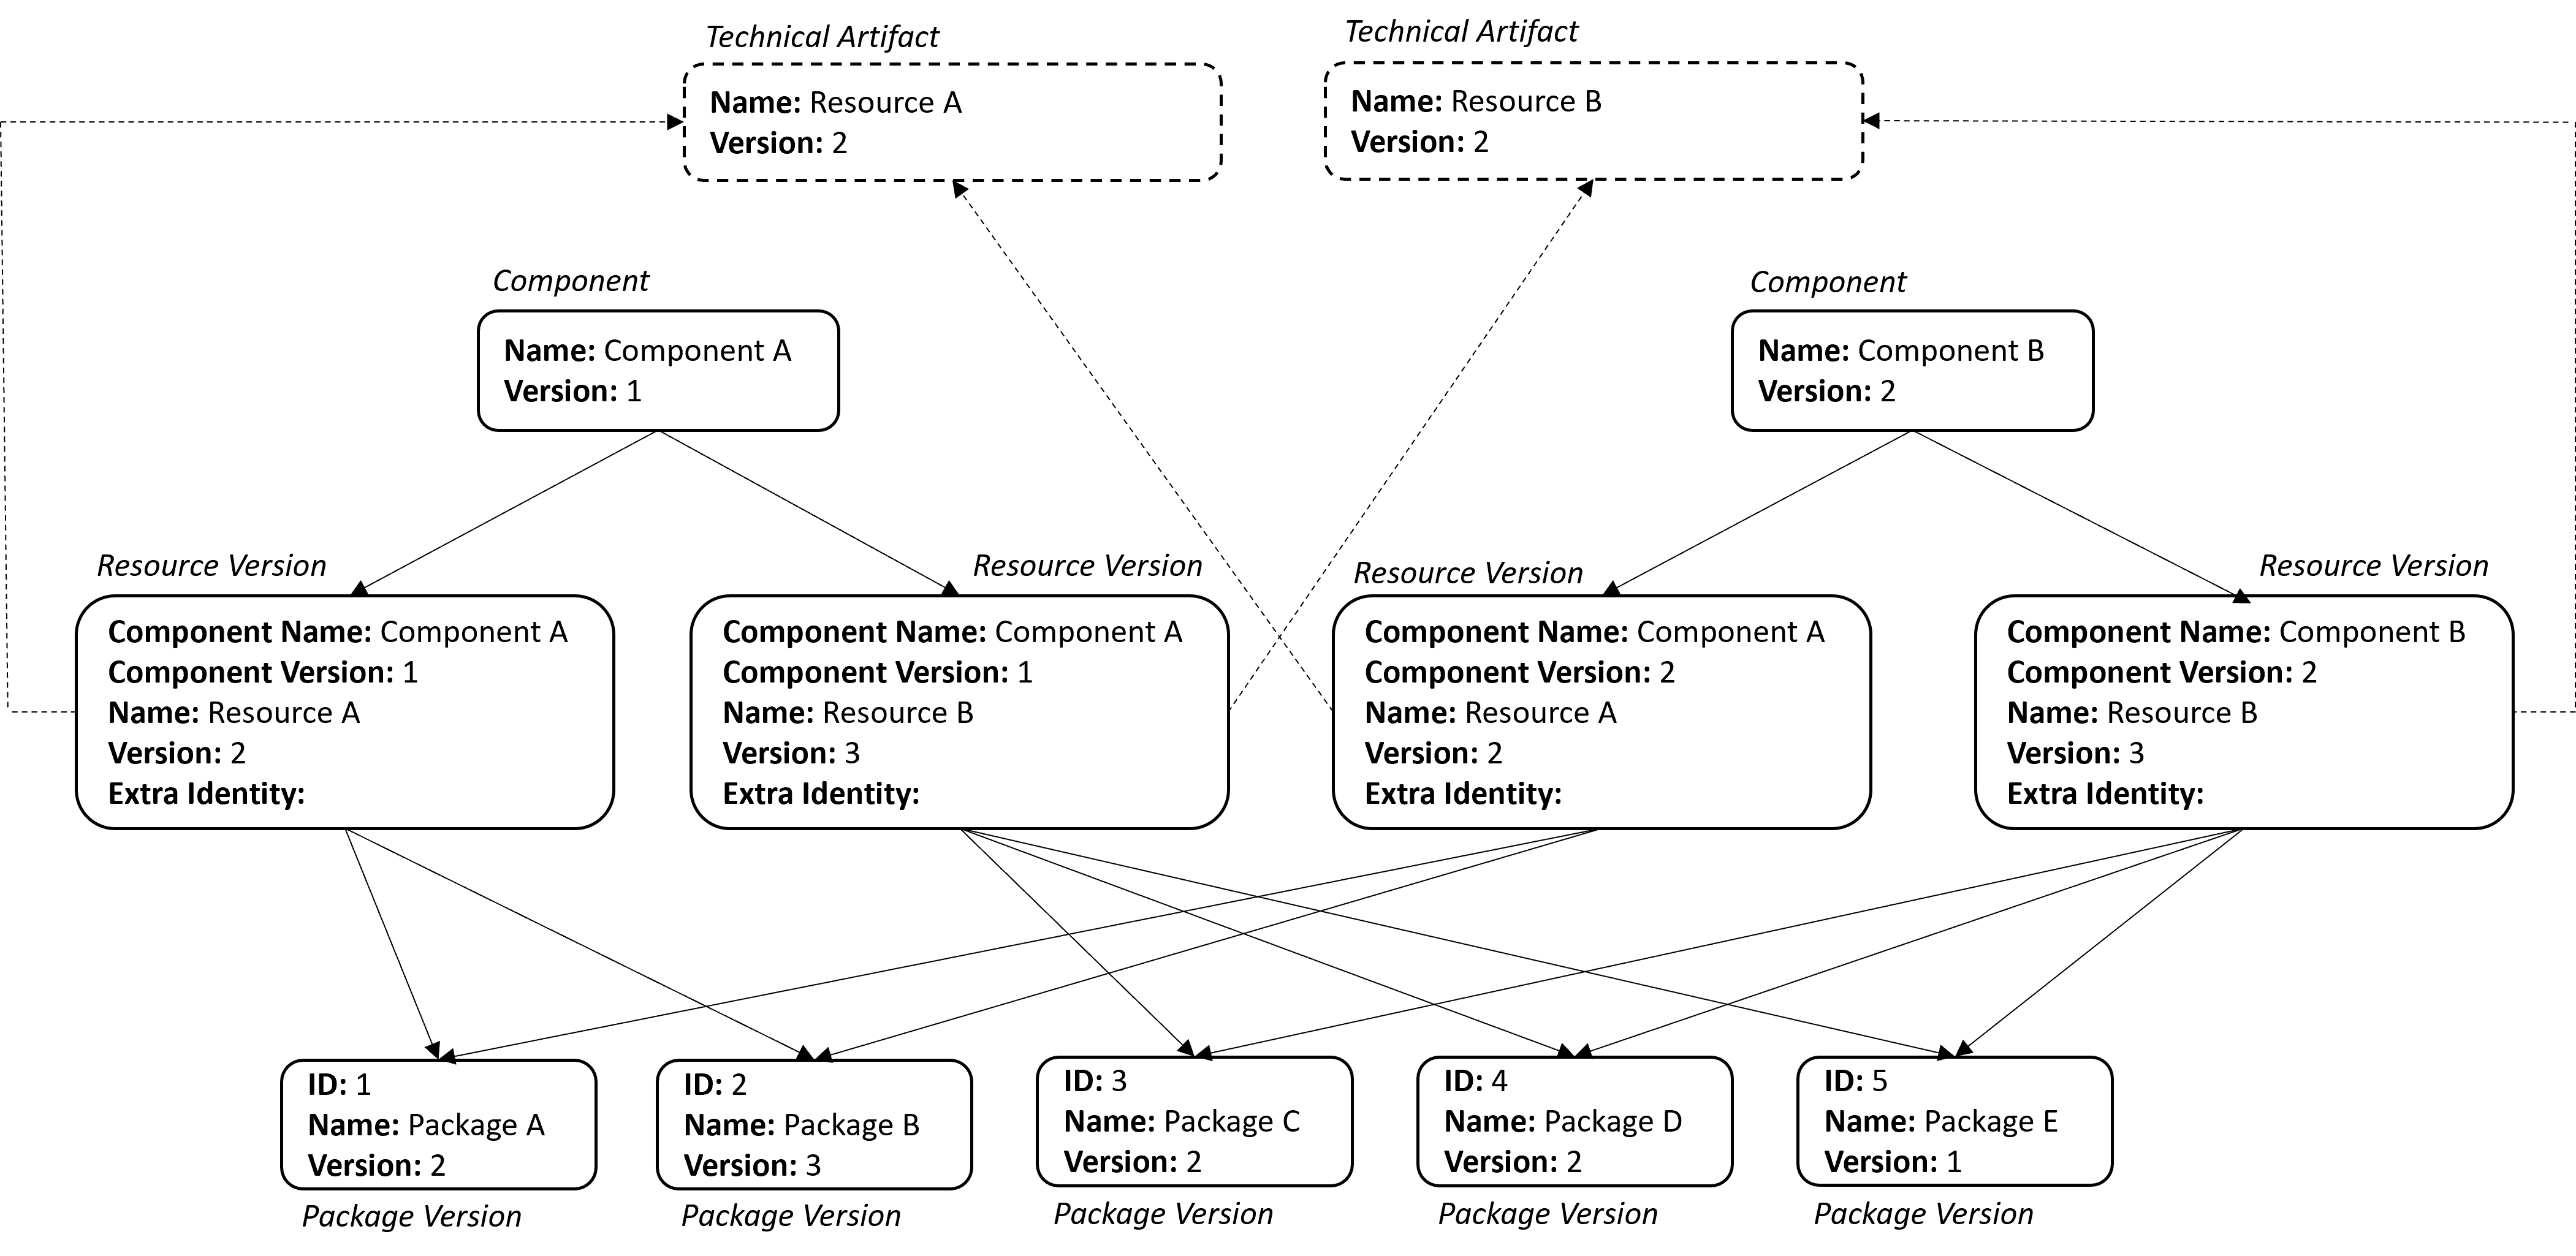
\includegraphics[scale=0.45]{localartifactidentity}
	\caption[Data Model]{Local Artifact Identities \source{Own Representation}}
	\label{fig:LocalArtifactIdentity}
\end{figure}

Figure \ref{fig:LocalArtifactIdentity} shows two components that reference the exact same technical artifacts. But since the \emph{Identity} of \emph{Resource Versions} is local, the component name and version are part of the \emph{Resource Versions Identity}, as also shown in figure \ref{fig:RefDataModel}. Thus, it appears as they are referencing different artifacts. But as the packages comprising the \emph{Resource Versions} are identified by scanning the technical artifact accessed through the access property, they are the same for the \emph{Resource Versions} which practically reference the same technical artifact.\par 
So, for answering questions such as which deployment contains Log4J and its corresponding vulnerabilities, the local artifact identities do not make a difference. As in practice, it may also be assumed that within a \emph{Component}, \emph{Resource Versions} with the same name but different version numbers are in fact pointing to different versions of the same technical artifact, the \emph{Resource} aggregate level is also kind of possible. But its scope and the scope of \emph{triage policies} within these entities respectively is of course limited to a certain \emph{Component}. Furthermore, attaching \emph{Build Information} and other \emph{Info Snippets} to artifacts is difficult with this approach.


\section{Database}
After the application context and data model are defined, a suitable database has to be selected. Therefore, this section analyzes the most relevant database technologies regarding their applicability as a central data store based on the previously defined data model.

\subsection{Requirements for the Database}
The most important aspect regarding the suitability of a database technology is the purpose of the data store and the respective kind of usage. Several relevant factors depend on this information. Is read or write performance more important? What may be acceptable delays when reading or writing data? What kind of queries may be used most frequently? Will the data be used for statistical analysis and require a lot of aggregation over dimensions such as time periods or locations? Are the entities highly inter-connected and require traversing relationships efficiently? How many users may need to access the data concurrently? May the database need to be distributed?\\\\
\textbf{Write Performance:} The data may be provided by all sorts of data sources. As already described in the reference architecture in section \ref{sec:Integration of the Security and Compliance Data Lake into the SAP Gardener Landscape} "Integration of the Security and Compliance Data Lake into the SAP Gardener Landscape", the data may be fetched based on policies. Considering scanning tools, such policies may require to scan all Component Versions or respectively the referenced technical artifacts once a day or based on particular events, such as upon creation of a new Component Version. Depending on the number and size of artifacts, the scans themselves take something between several minutes up to several hours. As the information in the database may be updated concurrently with the scanning process, so for example every time the scanning tool has finished scanning a particular artifact, the results may be fetched, the \emph{write performance may be quite low}. Theoretically, the database could correspondingly to the scanning tools take up to several minutes to write or update the information about an artifact.\\
\textbf{Read Performance:} As already pointed out in section \ref{sec:Non-functional Requirements} "Non-functional Requirements", the Security and Compliance Data Lake may prospectively be used as backend for dashboard web applications. Of course, these dashboards are for technical professionals. Thus, the response time does not necessarily need to abide to common UX design requirements, but still common queries should ideally not take more than several seconds. So \emph{read performance should be high}.\\
\textbf{Queries:} The most popular example for a query is "Which deployments contain Log4J?" or more precisely in terms of the previously introduced data model "Which Component Versions contain a vulnerable Log4J Package Version?" or even "Which Component Versions contain the Log4J Vulnerability?". Considering the exemplary data model in figure \ref{fig:RefDataModel}, to resolve this query, one has to find the \emph{Vulnerability} with \emph{CVE} \textit{CVE-2021-44228} \cite{Log4jVuln}, find all \emph{Package Versions} that contain this \emph{Vulnerability} and also all \emph{Package Versions} that directly on transitively depend on one of those \emph{Package Versions}, find all \emph{Source} and \emph{Resource Versions} that contain one of the respective \emph{Package Versions} and finally find all \emph{Component Versions} that reference one of the respective \emph{Artifacts}. Thus, resolving this query requires traversing a lot of relationships. This is probably also the most popular kind of query in general. Queries including aggregations may be something like "What Vulnerability contained in a Deployment X has the highest CVSS?". Therefore, even the queries including aggregation require a traversal of relationships to retrieve the subset of data the aggregation function has to be applied to.\\
\textbf{Distribution:} The database is the central metadata store of a company which is used to monitor the application landscape and increase the transparency of the infrastructure. Therefore, the number of concurrent users will not be exceedingly high. Besides, the whole application and thus, also the underlying database is not business critical for a company. So database distribution to increase scalability in terms of parallel queries or to increase availability and fault tolerance are not a primary concern for the Security and Compliance Data Lake.\\\\
From here on, this rough overview provides a good idea of the most important properties to consider when selecting a database technology for the Security and Compliance Data Lake. 



\subsection{Relational Databases}
The first database technology analyzed are \textit{relational databases}. They are by far the most popular and widely used database technology. This is represented in Stack Overflow's 2021 developer survey \cite{StackoverflowDeveloperSurvey}. There, the top 3 most used databases are MySQL, PostgreSQL and SQLite, which are all relational databases. Among the technologies discussed in detail here, it also has been around for the longest as the original paper introducing the relational model for databases by Edgar Codd was published in 1970 \cite{RelationalDatabaseOriginalPaper}. Therefore, the technology itself is very mature and there is a lot of know-how in the industry. Thus, relational databases are worth considering for every enterprise project.

\subsubsection{Theoretical Foundations} \label{sec:Theoretical Foundations Relational Database}
A quick repetition of the foundations of relational databases. The name "relational database" stems from the mathematical definition of relation: 

\begin{quote}
	\textit{Given sets S1, S2,..., Sn (not necessarily distinct), R is a relation on these n sets if it is a set of n-tuples, the first component of which is drawn from S1, the second component from S2, and so on. More concisely, R is a subset of the Cartesian product S1 × S2 x . . . × Sn.}
	\cite{RelationalDatabaseModel}
\end{quote}

Thus, a mathematical relation is an unordered set of tuples of the same type. Mapping this to the relational model, a table represents a relation, each row represents a tuple of this relation, the ordering of the rows is irrelevant and as per definition of sets, all rows are distinct from one another \cite{RelationalDatabaseModel}.\par
These relations are then used to represent objects of a certain problem domain, therefore entities and their relationships. Each object type has a distinct type identifier, which becomes the name of the relation. Every instance of an object type must have an instance identifier, which uniquely identifies the entity among all the other entities of the same type. This identifier is commonly referred to as primary key \cite{RelationalDatabaseModel}.\par
Relationships between entities are mapped to relations by using the primary key of a related entity as a reference. In the scope of the referencing relation, the primary key of the referenced relation is commonly referred to as foreign key \cite{RelationalDatabaseModel}.\par
Furthermore, the relations are usually normalized, which leads to a low level of redundancy and reduces the risk for anomalies during data manipulation, thereby enabling the adherence to the ACID criteria \cite{RelationalDatabaseModel}.\\\\
In order to being able to consider and compare performance, a basic understanding of how the data is stored and accessed with each database technology is required. For relational databases, these basics are explained excellently and with attention to detail by Ramez Elmasri and Shamkant Navathe in "Fundamentals of Database Systems" \cite{DatabaseFundamentals}. Based on this book, the most important principles which are also necessary for further understanding are introduced.\par
The data stored on disk is organized as \emph{files} of \emph{records}. Generally, a record is a collection of data values that can be interpreted as facts about entities, their attributes, and their relationships. In the context of relational databases, a record usually refers to a tuple of a relation, or respectively to a row in a table. Thus, the data is stored in a 1-dimensional format, listing all rows of a table.\par
There are several techniques, determining how the file records are physically placed on the disk, and hence how the records can be accessed. These techniques are commonly referred to as \emph{file organizations} or \emph{primary file organizations}. A \emph{heap file} or \emph{unordered file}, as the name suggests, places the records on disk in no particular order by appending new records at the end of the file. Opposed to that, a \emph{sorted file} or \emph{sequential file} keeps the records ordered by the value of a particular field called the \emph{sort key}. Correspondingly, a \emph{hashed file} uses a hash function applied to a particular field called the \emph{hash key} to determine a record's placement on disk. \emph{B/B\textsuperscript{+}-trees} use tree structures. \emph{Secondary file organizations} enable efficient access to file records based on \emph{alternate fields} than those that have been used for primary file organization.\par
The implications are quite intuitive. In the case of heap files, without additional indexing, thus secondary file organizations, a \emph{linear search} looking through each record has to be conducted when searching based on a specific condition. Even with file organizations and indexing, this is still the case for conditions only considering non-key fields \cite{DatabaseFundamentals}.\par 
As common relational database technologies such as InnoDB, the storage engine behind MySQL and MariaDB, use B\textsuperscript{+}-trees for both, primary as well as secondary file organization, this is discussed in further detail \cite{InnoDB}.

\begin{figure}[H]
	\centering
	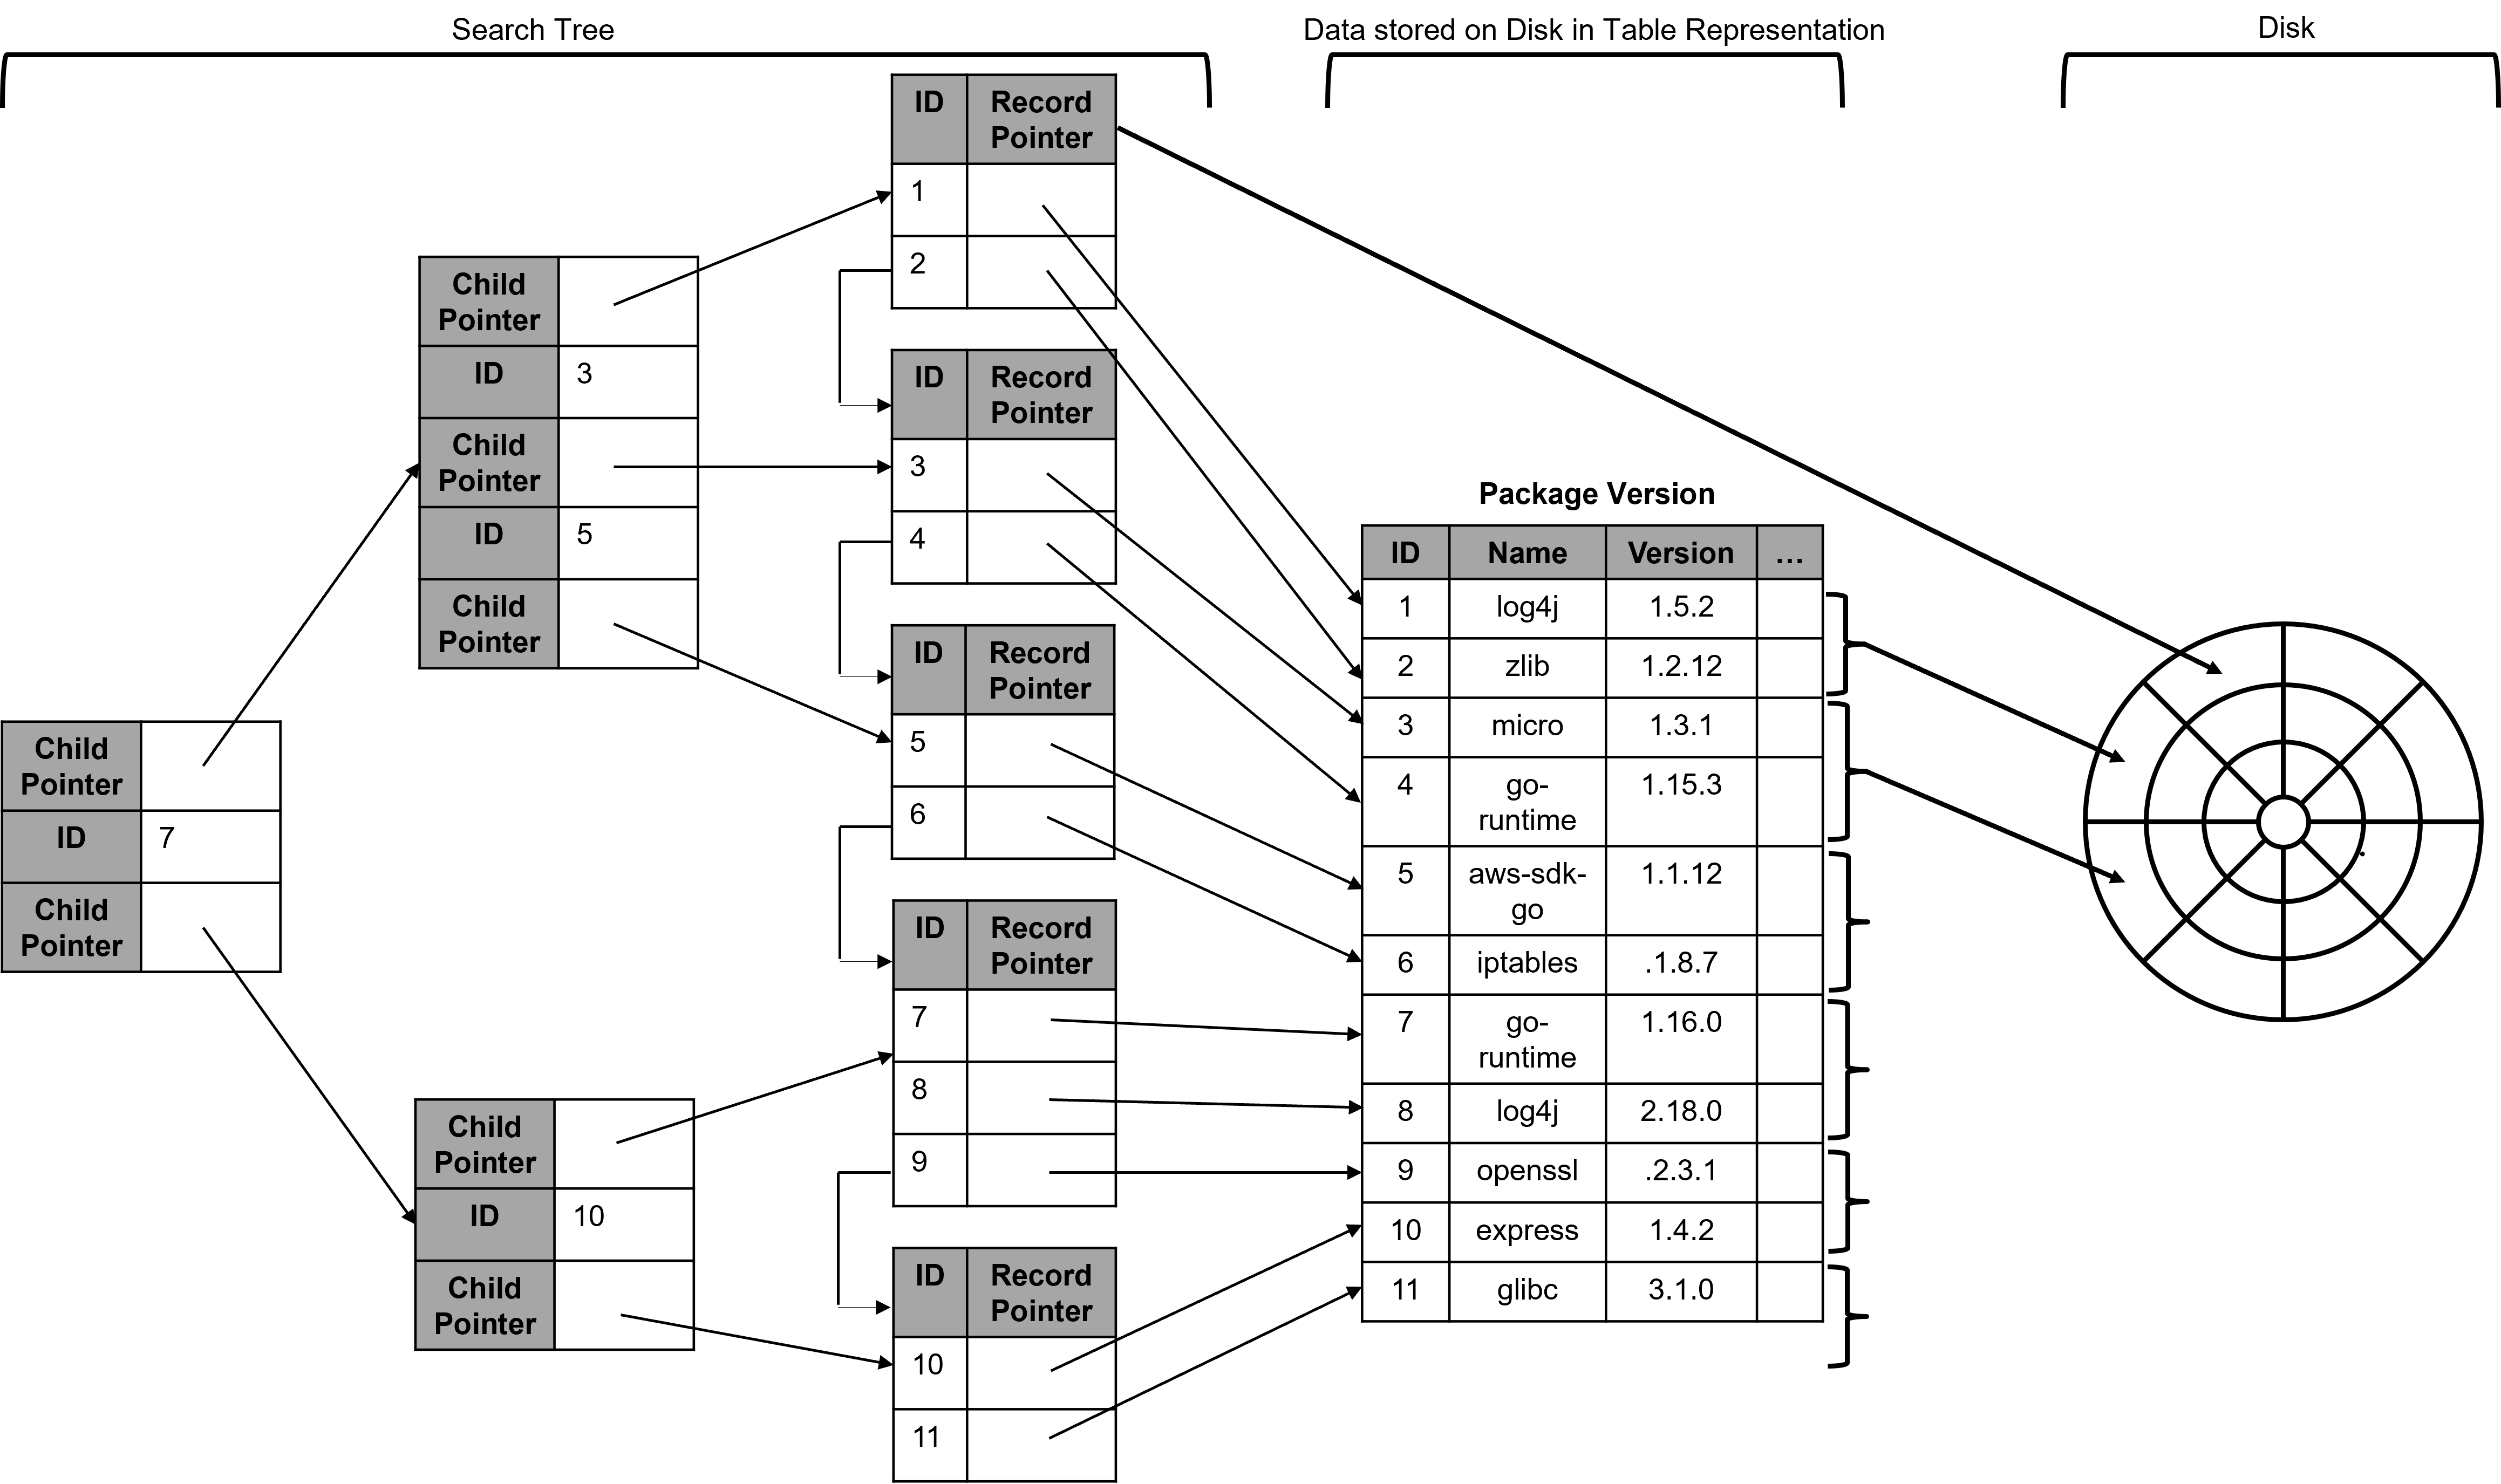
\includegraphics[scale=0.40]{Btree}
	\caption[B\textsuperscript{+}-tree as 4-way Search Tree]{B\textsuperscript{+}-tree as 4-way Search Tree \source{Based on \cite{DatabaseFundamentals}}}
	\label{fig:B+tree}
\end{figure}

So, figure \ref{fig:B+tree} provides a holistic view onto the search trees and how they are used in database systems. There are of course some simplifications and assumptions.\par 
On the right of the figure is a representation of a magnetic disk, which is still most commonly used as storage for large databases. The concentric circles are called tracks. These tracks are further divided into sectors, represented by the intersections of the concentric and straight lines. This division leads to equal-sized \emph{disk blocks}\footnote{One may wonder that these blocks are not equal sized in the figure. The outer ones are actually much larger than the inner ones. In practice, there are different types of sector organization. The type shown in the picture maintains a fixed angle. To provide equal-sized disk blocks nonetheless, the outer sectors usually have a lower record density \cite{DatabaseFundamentals}} which are also commonly called \emph{pages}. The pages are the areas the arrows are pointing to in the figure. With InnoDB, the block size may be configured between 4KB and 64KB.\par 
Data in secondary storage such as a disk cannot be processed directly by the \emph{central processing unit (CPU)}. First, it must be copied into a primary storage such as main memory which is usually \emph{dynamic random access memory (DRAM)}. The units in which this data is transferred between disk and main memory are the just introduced pages. Thus, to read data contained in a certain page, the whole page is copied into the main memory. And to change that data, this data is edited and then the whole page is written back, or in other words copied, to the disk. As accessing pages on the disk is in the order of milliseconds while accessing RAM is in the order of nanoseconds, this is a major bottleneck and therefore, the goal is to \emph{minimize the number of block transfers}. So this enables to understand the necessity of multilevel indexes or search trees.\par
By only looking at figure \ref{fig:B+tree} without the background knowledge just provided, there would be no apparent reason to construct and store such a sophisticated search tree. It would be more efficient to just store the index as a sorted table. Then, when accessing the database with said index, load the whole table into main memory and conduct a binary search. Thus, the only reason to use such search trees is when the index itself outgrows the page size and therefore has to be stored in multiple pages. So in practice, each node of a search tree is stored in a separate page as indicated by the arrow from the upper index leaf node. By traversing this search tree, the number of necessary page accesses may be reduced significantly. The index size with a search tree of order 4, so a node can at most have 4 children, is probably the most obvious simplification in above figure. The node and leaf indexes are so small that they could easily be stored together in a single index table.\par 
The example shows the search tree as used for secondary file organization. So the records could generally be stored as a heap file, with no ordering at all. If used for primary file organization, instead of having pointers to the actual records, the leafs would directly store the records enforcing a respective order.\par
To traverse such a search tree, lets assume to find the record with ID 4, one starts at the root node. This is the node illustrated on the far left. As 4 < 7, one follows the pointer above the 7 to the corresponding child node. In practice, this is a pointer to the page of the child node and consequently leads to copying this page into main memory. Then, this process repeats, as 3 < 4 < 5, one follows the pointer between 3 and 5 to the next child node. In this example, this is already a leaf node, containing the pointer to the actual record with ID 4. So here, 4 pages have to be loaded, 3 index pages and the page containing the actual record.\par
So up until now, instead of B-tree or B\textsuperscript{+}-tree, the term search tree was used. This is because B/B\textsuperscript{+}-trees are essentially search trees which have to abide to an extra set of constraints. To be more concrete, a \emph{B-tree of order m} is a tree which satisfies the following properties \cite{SortingSearchingBible}.

\begin{quote}
	\begin{enumerate}
		\item\textit{Every node has at most m children. }
		\item\textit{Every node, except for the root and the leaves, has at least $\lceil m/2 \rceil$ children}
		\item\textit{The root has at least 2 children (unless it is a leaf).}
		\item\textit{All leaves appear on the same level}
		\item\textit{A nonleaf node with k children contains k-1 keys}
	\end{enumerate}
\end{quote}

The goals of \emph{balancing}, which is another term for all leafs nodes being on the same level, is to make the search speed uniform. Thus, the average time to find any random key is roughly the same. Furthermore, these constraints ensure that the nodes stay relatively full and do not end up empty if there are many deletions, thereby preventing the waste of storage space and an unnecessary high number of levels.\par 
Figure \ref{fig:B+tree} shows a B\textsuperscript{+}-tree. A B\textsuperscript{+}-tree is actually a variation of a B-tree which stores record pointers only at the leaf nodes. Consequently, the leaf nodes have an entry for every ID leading to some IDs -- specifically 7, 3, 5 and 10 -- being contained twice in the search tree. On the contrary, in a B-tree every ID is only present once at some level in the tree and the record pointer is stored directly alongside the child pointers. Thus, in above figure, the root node would additionally have a pointer to the record with ID 7. But of course, the whole tree structure would be different, as several leaf nodes could be omitted. Furthermore, B\textsuperscript{+}-trees usually link the leaf nodes to provide ordered access. This is indicated by the the arrows between the leaf nodes. In practice, this linking is also done with an additional pointer \cite{DatabaseFundamentals}.\\\\
Finally, the \emph{upper bounds on running time} for searches with B-trees is examined. Initially, it is important to understand, the leaves carry essentially no information searching wise. Thus, for this considerations, leaves may just be regarded as terminal nodes. As explained in Donald Knuth's "Art of Computer Programming - Sorting and Searching" \cite{SortingSearchingBible}, suppose there are \emph{N} keys, and the \emph{N+1} leaves appear on level \emph{l} (In the book the relation that a B-tree with \emph{N} keys always has \emph{N+1} leaves is just given. For a further explanation on why this is always the case, refer to appendix \ref{apx:Relation of Number of Keys and Number of Leaves in a B-tree}). Then, as per constraint, the number of nodes on levels 1,2,3, ... is at least $2$, $2 \lceil m/2 \rceil$, $2 \lceil m/2 \rceil ^2$, ..., hence
$$ N + 1 \geq 2 \lceil m/2 \rceil ^l-1 $$
Solving the equation for l
$$ l \leq 1 + log_{\lceil m/2 \rceil}(\frac{N + 1}{2}) $$
Furthermore, on every level at most $m$ keys have to be searched. As the elements in the nodes of a B-tree are sorted, binary search my be used. Therefore, the maximum number of look ups $s$ per level is $log_2(m)$. Consequently, the total number of look ups is 
$$ s \leq \lceil (1 + log_{\lceil m/2 \rceil}(\frac{N + 1}{2})) \rceil * log_2(m) $$ 
Considering Big O notation, constants may be ignored. Also $m$ is definitely smaller than and independent of $N$. This leads to a worst case time complexity for searching a B-tree of 
$$ O(log N) $$ 
The estimation is also true for B\textsuperscript{+}-trees.\footnote{Although this section covers several details, it is still just a very brief introduction into relational databases, the internals of database systems and B-trees, only covering the topics in the depth necessary for understanding the further sections. Aspects such as transactions and ACID criteria, how the records are actually placed on the disk, how variable-length fields are handled or what happens when records exceed page boundaries have been omitted. Regarding B/B\textsuperscript{+}-trees, the algorithms used for insertion or deletion and their respective bounds on running time are not discussed either. For further and more detailed information on these topics, refer to the respective sources "The Relational Model for Database Management" \cite{RelationalDatabaseModel}, "Fundamentals of Database Systems" \cite{DatabaseFundamentals} and "The Art of Computer Programming - Searching and Sorting" \cite{SortingSearchingBible}.}

\subsubsection{Suitability for the Central Metadata Store}
To evaluate and properly illustrate the suitability of the database technology regarding the aforementioned relevant properties, a representative example based on the established data model is used. The complete data model is quite complex and its actual instantiated form, thus the final entities, relationships and especially the properties, depends on the use case. Therefore, to keep the considerations general and clear, the representative example only considers the \emph{Package Version} entity type. Since \emph{Package Versions} may be contained in other \emph{Package Versions} this example allows for considering arbitrarily complex relationship chains.\par

\begin{figure}[H]
	\centering
	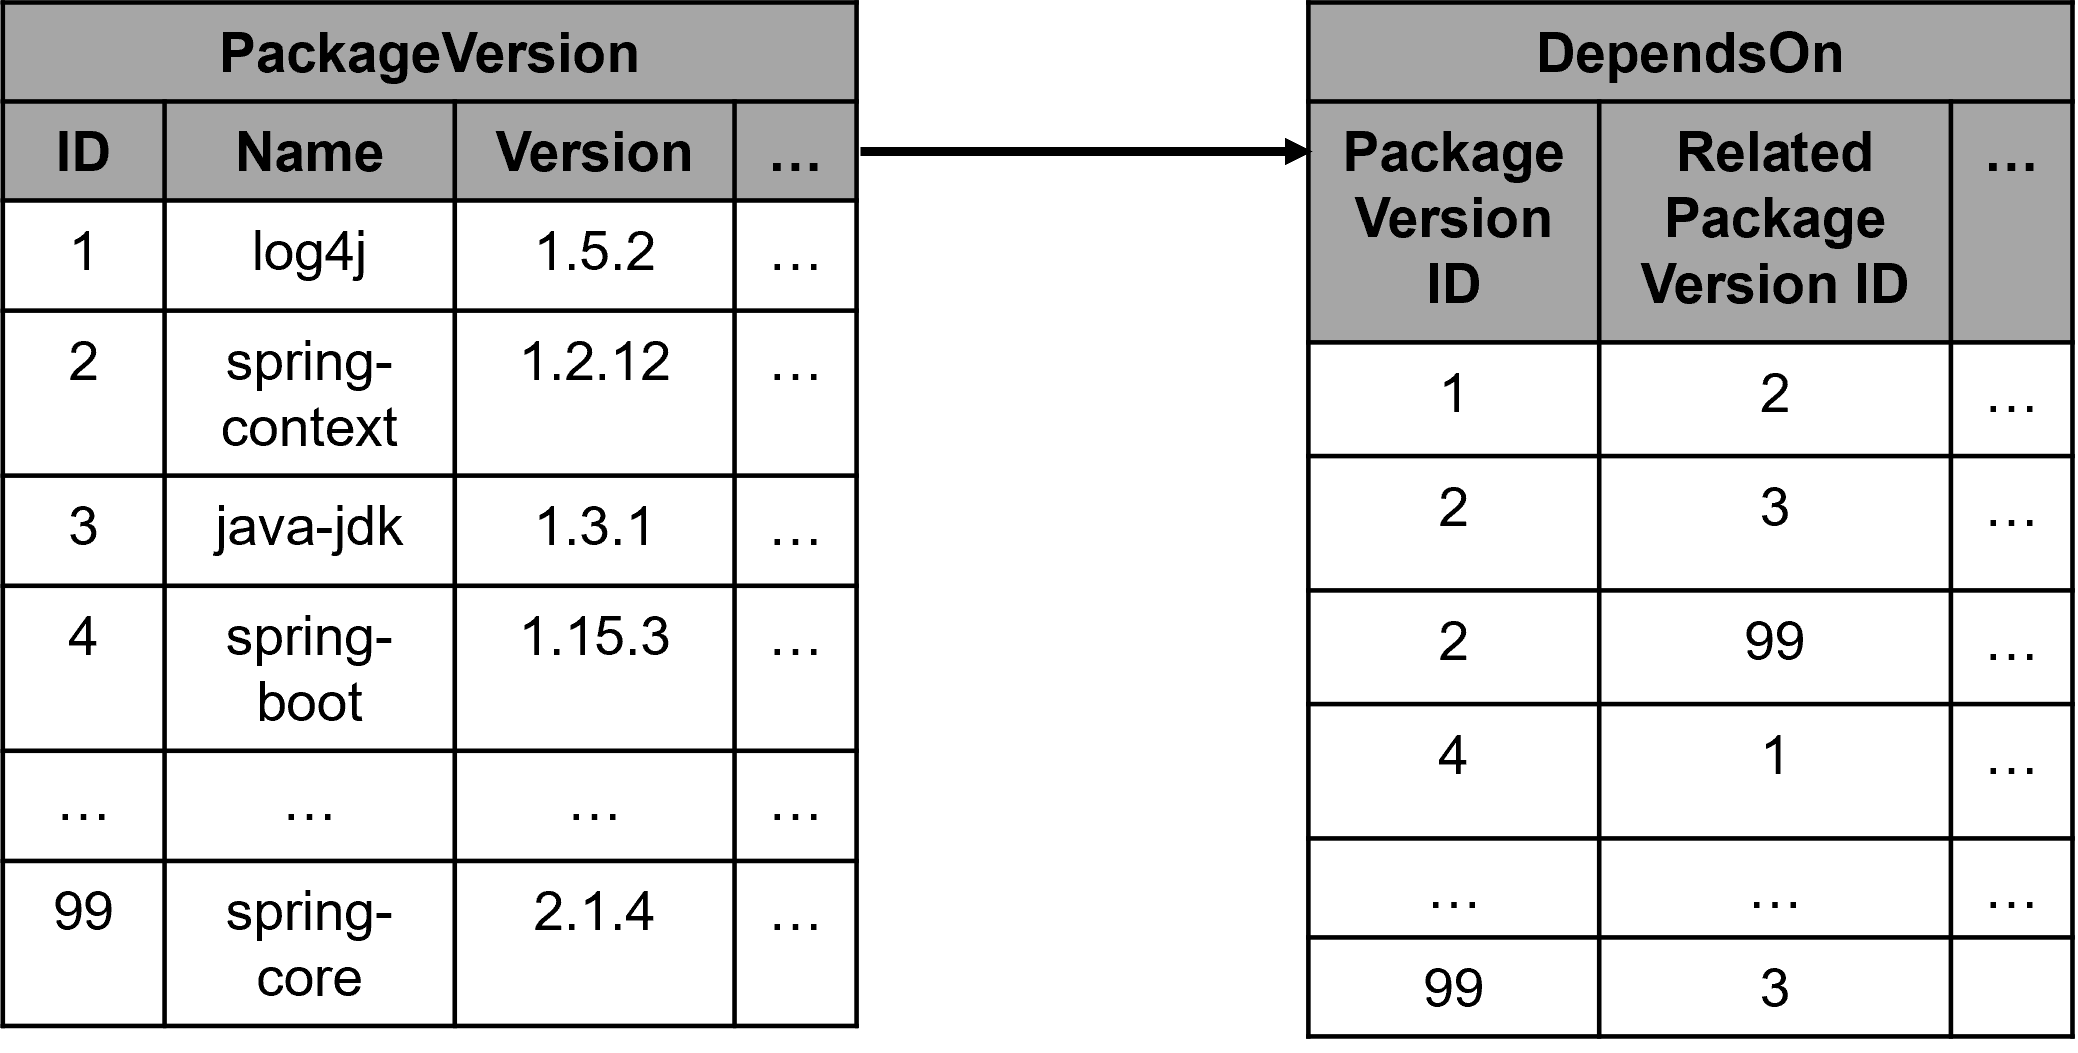
\includegraphics[scale=0.70]{friendsoffriends}
	\caption[Package Versions and Dependencies]{Package Versions and Dependencies \source{Based on \cite{neo4j}}}
	\label{fig:PackageVersionsAndDependencies}
\end{figure}

Figure \ref{fig:PackageVersionsAndDependencies} shows the \emph{Package Version} entity type and the corresponding \emph{depends on} relationship type mapped to tables and filled with some example entities.  As indicated by the ordering of the tables, the example also assumes there are indexes on \emph{ID} and \emph{PackageVersionID}. Furthermore, it may also be assumed, that there is a composite index on \emph{Name} and \emph{Version}.\par
For simplicity reasons, initially pretend there are no transitive dependencies. In this case, to answer the question "Which Package Versions does the spring-context:1.2.12 Package Version depend on?" in relational database, the following SQL query would have to be used:

\begin{lstlisting}[language=SQL, caption=Package Version Dependencies, captionpos=b, label=lst:PackageVersionDependencies]
SELECT p1.Name, p1.Version
  FROM PackageVersion p1 
  JOIN DependsOn
    ON DependsOn.RelatedPackageVersionID = p1.ID
  JOIN PackageVersion p2
    ON DependsOn.PackageVersionID = p2.ID
 WHERE p2.Name = "spring-context" AND p2.Version = "1.2.12"
\end{lstlisting}

Based on the sample data in figure \ref{fig:PackageVersionsAndDependencies}, this returns \emph{java-jdk 1.3.1} and \emph{spring-core 2.1.4} \cite{neo4j}. Although slightly hard to read, the query is still relatively simple and not particularly computationally expensive, because it constraints the number of rows under consideration by applying the filter \lstinline|WHERE p2.Name = "spring-context" AND | \lstinline|p2.Version = "1.2.12"|. Based on the indexes, this initial look up of this record has a time complexity of $O(log(n))$ with $n$ being the number of rows in the PackageVersion table. The consecutive join then has a time complexity of $O(m*log(n))$ with $m$ being the number of records found during the previous look up and $n$ being the number of rows in the DepensOn table. Each additional join in the query adds a $O(m*log(n))$. This assumes the so called nested loop join algorithm is used. This is usually the most efficient join algorithm in such scenarios, where indexes on the join condition exist and it is a small number of rows that have to be joined. Relational databases automatically estimate and choose the best strategy \cite{PostgreSQLJoin}. Thus, depending on the number of joins, the general time complexity for such a relationship traversal query may be estimated as 
$$O(log(n)) + O(m*log(n)) + ... + O(m*log(n))$$ 

Now, to answer the reciprocal question "Which Package Versions depend on the spring-context:1.2.12 Package Version?" in a relational database, the following SQL query would have to be used:

\begin{lstlisting}[language=SQL, caption=Package Version Reciprocal Dependencies, captionpos=b, label=lst:PackageVersionReciprocalDependencies]
SELECT p1.Name, p1.Version
  FROM PackageVersion p1 
  JOIN DependsOn
    ON DependsOn.PackageVersionID = p1.ID
  JOIN PackageVersion p2
    ON DependsOn.RelatedPackageVersionID = p2.ID
 WHERE p2.Name = "spring-context" AND p2.Version = "1.2.12"
\end{lstlisting}

Based on the sample data in figure \ref{fig:PackageVersionsAndDependencies}, this returns \emph{log4j 1.5.2} \cite{neo4j}. Although this query looks very similar to the one before, it is computationally much more expensive, because there is no index on \emph{RelatedPackageVersionID} and consequently, the whole table has to be considered with a complexity of $O(n)$. In practice, an additional index could be added without problems, as the write performance which would suffer from maintaining an additional index, does not matter too much in this use case.\\\\
Finally, the transitive dependencies have to be considered. To traverse these transitive dependencies in SQL, recursive joins have to be used. Therefore, joining a table with itself. But as the dependency chains may be of arbitrary length, a simple recursive query is not sufficient. Nowadays, most of the popular relational database provide a SQL feature, the WITH clause or rather \emph{Common Table Expressions (CTE)}, to support recursive queries \cite{mysqlCTE, postgresCTE, sqliteCTE}. CTEs are auxiliary statements which can be thought of as defining temporary tables existing for just one query \cite{postgresCTE}. So to actually answer the question "Which Package Versions does the spring-context:1.2.12 Package Version depend on?" correctly, thus also including the transitive dependencies, the following SQL query would have to be used:

\begin{lstlisting}[language=SQL, caption=Package Version Dependencies (including transitive), captionpos=b, label=lst:PackageVersionDependenciesIncTransitive]
WITH RECURSIVE cte(PackageVersionID) AS (
  -- Anchor member.
  SELECT d.RelatedPackageVersionID
    FROM DependsOn d
    JOIN PackageVersion p
      ON d.PackageVersionID = p.ID
   WHERE p.Name = 'spring-context' AND p.Version = '1.2.12'
  UNION ALL
  -- Recursive member.
  SELECT d.RelatedPackageVersionID
    FROM DependsOn d
    JOIN cte
      ON d.PackageVersionID = cte.PackageVersionID
)

SELECT p.Name, p.Version
  FROM PackageVersion p
  JOIN cte
    ON cte.PackageVersionID = p.ID
\end{lstlisting}

Based on the sample data in figure \ref{fig:PackageVersionsAndDependencies}, this returns \emph{java-jdk 1.3.1} twice (as union all does not remove duplicates) and \emph{spring-core 2.1.4}. And correspondingly to answer reciprocal question "Which Package Versions depend on the spring-context:1.2.12 Package Version?", the following SQL query would have to be used:

\begin{lstlisting}[language=SQL, caption=Package Version Reciprocal Dependencies (including transitive), captionpos=b, label=lst:PackageVersionReciprocalDependenciesIncTransitive]
WITH RECURSIVE cte(PackageVersionID) AS (
  -- Anchor member.
  SELECT d.PackageVersionID
    FROM DependsOn d
    JOIN PackageVersion p
      ON d.RelatedPackageVersionID = p.ID
   WHERE p.Name = 'spring-context' AND p.Version = '1.2.12'
  UNION ALL
  -- Recursive member.
  SELECT d.PackageVersionID
    FROM DependsOn d
    JOIN cte
      ON d.RelatedPackageVersionID = cte.PackageVersionID
)

SELECT p.Name, p.Version
  FROM PackageVersion p
  JOIN cte
    ON cte.PackageVersionID = p.ID
\end{lstlisting}

Based on the sample data in figure \ref{fig:PackageVersionsAndDependencies}, this returns \emph{log4j 1.5.2} and \emph{spring-boot 1.15.3}. The queries are tested with a PostgreSQL 15 database. The respective DDL statements to set up the sample data are included in appendix \ref{apx:Data Definition Statement for SQL Sample Data}.\par
Besides the computational complexity and the general difficulty of the queries, another aspect to consider are the \emph{schemas} required by relational databases. This may lead to a lot of null values in a table in cases where data sources do not provide the same amount of information for entities of the same type. Depending on how the data is stored on disk, this may lead to a waste of storage space.\\\\
So, as a conclusion for this section, a quick summary of the most important aspects when considering a relational database for the use case. 
(n:m)-relationships lead to large tables in relational databases. To be able to efficiently traverse these relationships and run queries with a reasonable performance, it is important to define \emph{indexes} on the columns used in the respective join conditions. Relational databases that support recursive CTEs are able to \emph{traverse hierarchies of arbitrary depth} without additional logic in the client side code. The \emph{queries to traverse several relationships become quite large and may be hard to read}. The so called \emph{row format}, thus, how a relational database stores records on disk, should be considered when configuring the database to avoid waste of storage space through null values. 
 
\subsection{Document Databases}
\emph{Document Databases} have grown tremendously in popularity throughout the last several years. Especially MongoDB which is ranked the top 4 most used database in Stack Overflow's 2021 developer survey has found widespread use as a primary database for applications and therefore, as a substitute for relational databases \cite{StackoverflowDeveloperSurvey}.

\subsubsection{Theoretical Foundation}
Document databases are a type of NoSQL database which commonly interpreted as an acronym for "Not only SQL". It thereby is somewhat of an extension of the most simplistic kind of databases, the key-value databases. These allow very fast look ups at the cost of only allowing users to address records by their key. The value is usually \emph{opaque} to the database. Correspondingly, document databases also do not require a schema for the values they store, but they store the values in a standard format such as XML, PDF or most frequently JSON \cite{NoSQL}. Hence, the values are not opaque and the database may still parse the data and create indexes on non-key fields even though being schema less.\\\\
Generally, the primary reason for using document databases, or rather any NoSQL databases, are the horizontal scalability issues of relational databases \cite{NoSQL}. While vertical scalability refers to providing the database machine with more compute resources, thus, CPU and RAM, horizontal scalability refers to distributing the database over multiple machines. The important questions at this point are, where do the scalability issues come from? And also, how are they overcome by document databases?\par
\emph{De-normalization} is one of the key features of document databases. Thus, while relational databases map entities and relationships to multiple tables connected by foreign keys, document databases allow storing entities and relationships as nested structures through their schema less nature. These nested structures are often referred to as \emph{documents} or also more generally \emph{aggregates}, a term from Domain-Driven Design describing a collection of related objects that is treated as a unit. Documents are grouped to \emph{collections}, which is kind of the equivalent to a table in relational database \cite{NoSQLDistilled}. A common example is shown by figure \ref{fig:NoSQLDataModel} and listing \ref{lst:JSONDocument}.\par 

\begin{figure}[H]
	\centering
	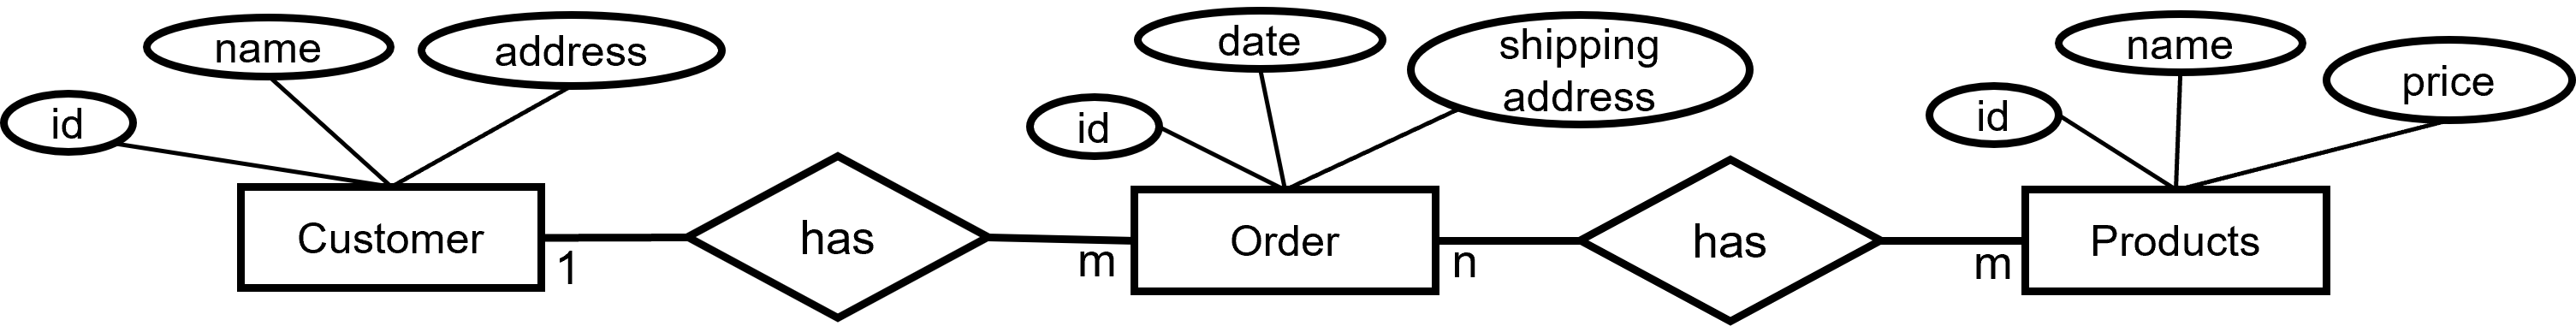
\includegraphics[scale=0.60]{no_sql_datamodel}
	\caption[Sales Data Model]{Sales Data Model \source{Based on \cite{NoSQLDistilled}}}
	\label{fig:NoSQLDataModel}
\end{figure}

\begin{lstlisting}[language=JSON, caption=JSON Document, captionpos=b, label=lst:JSONDocument]
{
  "id": 1,
  "name": "Martin",
  "address": 
    {"city": "Berlin"}
  "orders": [
    {"id": 99,
     "date": "04.01.2023",
     "shippingAddress": {"city": "Berlin"}
     "products": [
       {"id": 42,
        "name": "The Hitchhiker's Guide to the Galaxy",
        "price": 7.50 },
       {"id": 12,
        "name": "The Art of Computer Programming",
        "price": 120.00 }
      ]
    }
  ]
}
...
\end{lstlisting}


This solves the so called \emph{impedance mismatch}, the difference between the relational model and in-memory data structures. Hence, with relational databases developers frequently have to translate the nested in-memory data structures to a relational representation to persist them. Of course, there are object-relational mapping frameworks such as Hibernate, but these often lead to performance issues \cite{NoSQLDistilled}. By allowing to store objects as JSON objects, document databases such as MongoDB enable developers to store and retrieve their \emph{JavaScript} objects or \emph{Python} dictionaries as they are, without any further conversion. This is definitely one of the major reasons for their success, also in use cases where scalability is not a primary concern.\par
Furthermore, through this de-normalization, document databases \emph{remove the necessity of joining a lot of data}. On one hand, this makes querying objects such as customer with all its orders easier for developers, as join queries are comparably difficult to write and understand. On the other hand, this increases the performance and scalability of this queries, as joins add quite some computational complexity which even depends on the number of stored objects. Thus, the performance of joins becomes worse as the database grows.\par
Besides, this kind of data organization enables efficient \emph{sharding}. Sharding is a technique where different parts of the data is put onto different severs. Tables or in the context of document databases rather collections, are split up into smaller shards which may be placed on multiple servers. A common sharding technique is to hash a key, also called \emph{shard key} in MongoDB \cite{MongoDBShardKey} or \emph{partition key} in DynamoDB \cite{DynamoDBPartitionKey}. The respective hash value determines where, so on which server, to place the shard. This hashing provides an even distribution. But there are also other techniques such as ranged sharding. Thereby, the shards are distributed by the key value itself. This may be useful, when the records have some sort of order and its common to access multiple sequential records. Or the key may be a post code and the distribution is based on the sever location to minimize latency \cite{NoSQLDistilled}. This whole technique is enabled through the nesting, as documents are collection of related objects that are treated as units. Therefore sharding, or generally any form of partitioning, is rather difficult with relational databases. Since the data is scattered over multiple tables and the query language SQL puts no restrictions on how to query and connect this data, such partitioning would regularly require to send requests over the network to collect all the information \cite{NoSQLDistilled}.\par 
So de-normalization obviously has numerous advantages. And this is also where most getting started guides of document databases such as MongoDB stop \cite{MongoDBGettingStarted}. But naturally, it introduces the issues which were solved by normalization in the first place. Considering the example above, there is a (n:m)-relationship between orders and products. As the product is nested in the order which is again nested within the customer, updating a particular product while maintaining data integrity requires searching through all customers and through all orders within those customers, to update every single occurrence. Of course, in some cases write performance may not be relevant. But the nesting also affects queries. Imagine the above example describes the database of a retailer and this retailer wants to analyze its "Hitchhiker's Guide to the Galaxy" product sales over the last year. Again, to do this, the database has to search through all orders within all customers. There is the option to create indexes on nested fields which works pretty similar to relational database indexes to increase this performance. The problem that remains in this case is that document databases still have to retrieve the entire documents that contain the respective product from disk. Thus, every customer record with all orders and all products. This leads to enormous RAM usage and may also slow down the performance significantly \cite{MongoDBAppliedDesign}.\\\\
Generally, there are several restrictions which may serve as an orientation whether to nest or embed documents or whether to normalize and link them. \par 
If the application frequently has to \emph{access the embedded document independently of the embedding document(s)} and the \emph{documents are quite large}, it may be best to normalize and link the document rather than embedding due to the otherwise excessive RAM usage \cite{MongoDBAppliedDesign}. In above example, orders may be queried independently of customers. So it may be better to normalize this and make the orders reference the respective customer.\par 
\emph{If documents grow, the database may have to relocate it on disk} to an area with more space. In the above example, as a customer may regularly order products from the retailer, the order array within the customer document would grow and potentially require relocation. Such a relocation decreases performance significantly \cite{MongoDBAppliedDesign}. Moreover, document databases may even have a \emph{hard limit for the document size}. For MongoDB, this limit is 16MB \cite{MongoDBDocumentSizeLimit}. So, this is another argument to normalize the orders.\par 
Considering all these limitations, many-to-many relationships are especially problematic to de-normalize. Therefore, MongoDB even suggests to \emph{model complex many-to-many relationships in normalized form} \cite{MongoDBDataModeling}. For simple many-to-many relationships, where the references may rarely be updated, it is also a possibility to embed the references instead of creating the equivalent of a join table.\par
As especially MongoDB and its query language provide a lot of the functionality also provided by SQL, the final question may be, why not store the relational model in a document database? The primary concern therefore may be data integrity. Although MongoDB provides ACID conform transactions, there is no way to enforce referential integrity on database level. Without a schema, there is no way to tell the database about foreign keys and corresponding constraints.\par Furthermore, several operations such as joining are usually more efficient with a relational database. The syntax to perform the join is also simpler with SQL. To make this more tangible, below listing shows the syntax to perform the logical equivalent to a left outer join on orders with products. The example thereby assumes the data is stored according to a relational model as shown in \ref{apx:Data Definition Statement for MongoDB Sample Data}. 

\begin{lstlisting}[language=JSON, caption=JSON Document, captionpos=b, label=lst:JSONDocument]
db.orders.aggregate([
{ "$match": { "_id": 1 } },
{ "$lookup": {
  "from": "relations",
  "let": { "orderId": "$_id" },
  "pipeline": [{"$match":{"$expr":{"$eq":["$order","$$orderId"]}}},
  { "$lookup": {
    "from": "products",
    "let": { "productId": "$product" },
    "pipeline": [{"$match":{"$expr":{"$eq":["$_id","$$productId"]}}}],
    "as": "products" }
  }],
  "as": "order_products" }
},
{ "$project": {
  "_id": 1,
  "date": 1,
  "shippingAddress": 1,
  "products": "$order_products.products" }
}
])
\end{lstlisting}

Without going into too much detail about this query, it is obvious that it is rather complex and resembles a query execution plan. Thereby, the output of each stage (\$match, \$lookup, \$lookup, \$project) is the input of the consecutive stage \cite{MongoDBAggrPipeline}. This drastically limits the automatic optimization capabilities. So MongoDB will generally always perform a nested loop join even without indexes when a relational database would probably perform a merge or hash join.\\\\ 
So document databases and de-normalization work especially well, in cases where the application only requires a limited set of specific repetitive access patterns. But in order to actually leverage the advantages, these access patterns have to be identified and the de-normalization has to be done accordingly. This requires a very good understanding of the application already in the data modeling phase.\footnote{Again, although this section covers several details about document databases, it is still just a very brief introduction to provide the foundations necessary for understanding the further sections. Especially the topics of transactions and ACID criteria as well as the CAP theorem and the general treatment of consistency in document databases have been omitted.} 

\subsubsection{Suitability for the Central Metadata Store}
In contrast to the corresponding section about the suitability of relational databases, this one is kept short. Based on the background knowledge provided in the theoretical foundations, it is apparent that the advantages of document databases may barely be leveraged for this use case. Extensive examples on how to implement the central metadata store with the capabilities of a document database are therefore omitted as well.\\\\ 
The data model is based on (n:m)-relationships. Also, the database primary purpose is to perform analysis about different entities. Thus, "Which Component Versions contain a vulnerable Log4J Package Version?" with Package Version being the access point. Or reciprocal, "Which Package Versions are contained in a particular Component Version?" with Component Version being the access point. So, there is not a limited set of specific repetitive access patterns as every entity may need be used as access point to answer common questions. Therefore, the \emph{central metadata store cannot really be optimized through de-normalization}.\par
Consequently, at least concerning the major entities, the data model would have to be stored as a relational model. In this case, the document database would have the same scalability issues as relational databases and thereby mitigate a lot of the general advantages of document databases. Relational databases are practically designed with the primary purpose of handling relational models. Consequently, the query language, SQL as well as the general data processing is better adjusted to such use cases.\par 
Besides, being \emph{schema less} is also not a really big advantage for this use case. Data integrity may not be enforced and at least parts of the data have to adhere to some schema, in order to being able to merge the data of different data sources. Generally, to increase data quality and queryability, a schema would be enforced on application level anyway.

\subsection{Graph Databases}
The last database technology analyzed are \emph{graph databases}. They are also a type of NoSQL database. Although especially Neo4j is doing a lot of advertising, graph databases are still the least known database technology, as also represented by their absence in Stack Overflow's 2021 developer survey \cite{StackoverflowDeveloperSurvey}.

\subsubsection{Theoretical Foundation}
The previous sections discussed the foundations of relational databases such as how the data is stored and how the common b-tree indexes work, thereby deducting the complexity of index based look ups and joins. As relational databases traverse relationships through joining records, this complexity provides a kind of measure for traversing relationships. Then relational databases have been compared to document databases, which work quite similar regarding indexes, look ups and join, but also provide the option to represent relationships through nested structures. Finally, this section examines graph databases, which take an entirely different approach of representing relationships between entities.\par
Again, first a quick repetition of the foundations. The mathematical definition of a graph is the following: 
\begin{quote}
	\textit{A graph is a pair of sets $G = (V,E)$. In an undirected graph, the elements of $E$ are 2-element subsets $\{v,w\}$ of $V$. In a directed graph, the elements of $E$ are 2-element tuples $(v,w)$, thus ordered pairs, of $V$.}
	\cite{IntroductionToAlgorithms}
\end{quote}
In this definition, $V$ refers to \emph{vertices}, or rather \emph{nodes}, and $E$ refers to \emph{edges}. Quite frequently, $v \epsilon S1$ and $w \epsilon S2$ with $V = S1 \cup S2$, thus, two nodes $v$ and $w$ connected through an edge $(v,w)$ are elements of different sets. So, $E$ is a subset of the Cartesian product of $S1 x S2$. Looking back at the definition of relations in section \ref{sec:Theoretical Foundations Relational Database} "Theoretical Foundations" of relational databases, this is also the definition of a relation.\par
Thus, $E$ is a \emph{relation} and $V$ is the union of the \emph{source set} and \emph{destination set}. Now, this is generally well known from functions, which are defined by a \emph{domain} $S1$, a \emph{codomain} $S2$ and a \emph{mapping} $f$, which assigns elements of $S1$ to elements of $S2$. Hence, drawing a function in a coordinate system is essentially the visualization of a graph, where commonly the \emph{x-axis} denotes the \emph{source set} and the \emph{y-axis} denotes the \emph{destination set} and the dots, or rather line, for most common functions denotes the \emph{relation}.\par
In practice with business data, the source set and the destination set are usually sets of discrete and finite elements and the relationship between them is rather artificial and application specific. A primitive example, $S1$ may be the set of all package names, $S2$ may be the set of all version numbers and the relation $E$ $(v, w)$ may be package versions. Thereby, the source set and destination set are rather irrelevant. Besides, one could argue that for the scope of an application, the union of all $v$ in $E$ is equal to the source set and the union of all $w$ in $E$ is equal to the destination set.

\begin{figure}[H]
	\centering
	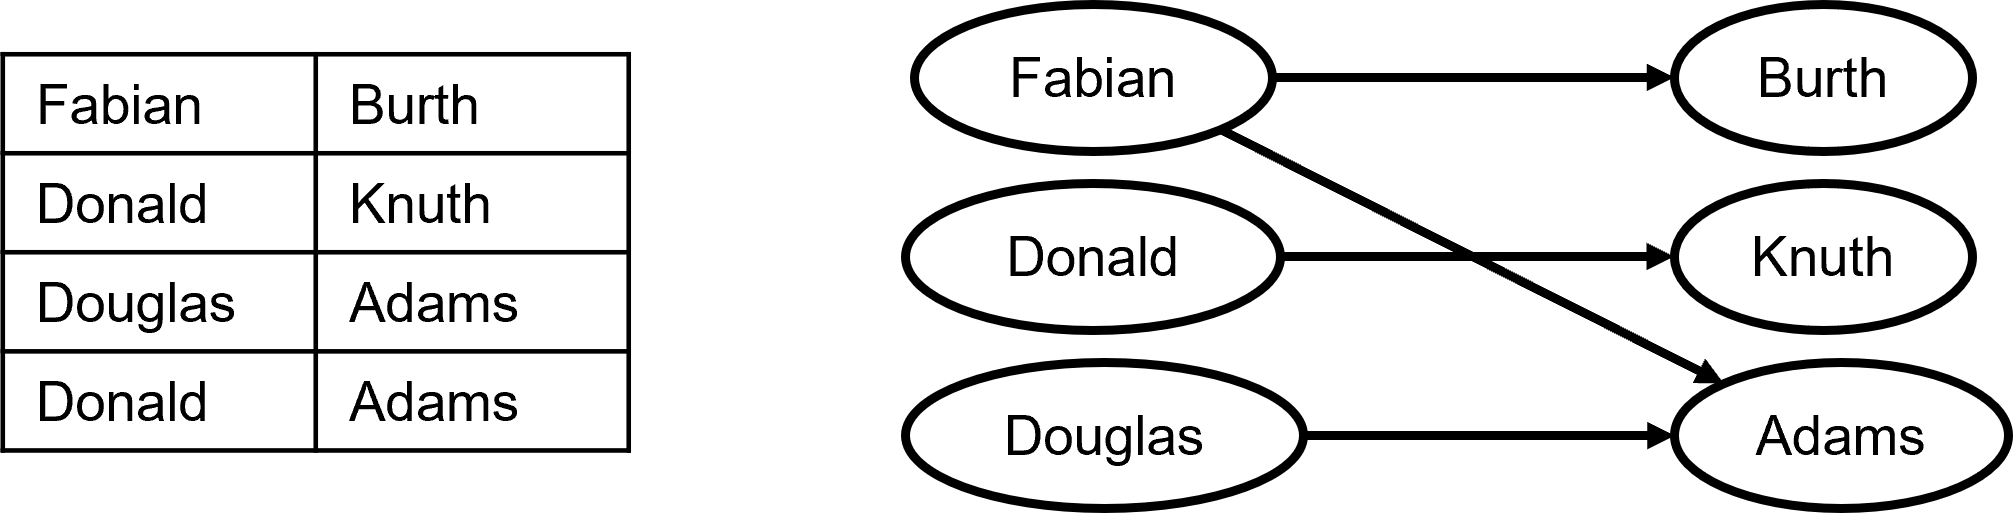
\includegraphics[scale=0.70]{table_vs_graph}
	\caption[graph representations]{Graph Representations}
	\label{fig:GraphTheoryExample}
\end{figure}

So, for the scope of an application, the table and the vertices and edges in figure \ref{fig:GraphTheoryExample} may be interpreted as two different representation of the same graph. This comparison of relations and graphs may be a slightly abstract and the example is oversimplified, but its purpose is to show how these two concepts and their common representations are tightly coupled.\\\\
The first part approached the topic from a mathematical perspective. From here on, this shifts to the actual technologies. Although the previous example may indicate this, in graph databases the graph is not used as a different representation for classical relations, hence to represent the relation of the properties of an entity. It is rather used to represent the relationships between the different entities. Thus, even though figure \ref{fig:GraphTheoryExample} is theoretically accurate, the following figure \ref{fig:GraphDBExample} is more suitable from a database technology perspective.

\begin{figure}[H]
	\centering
	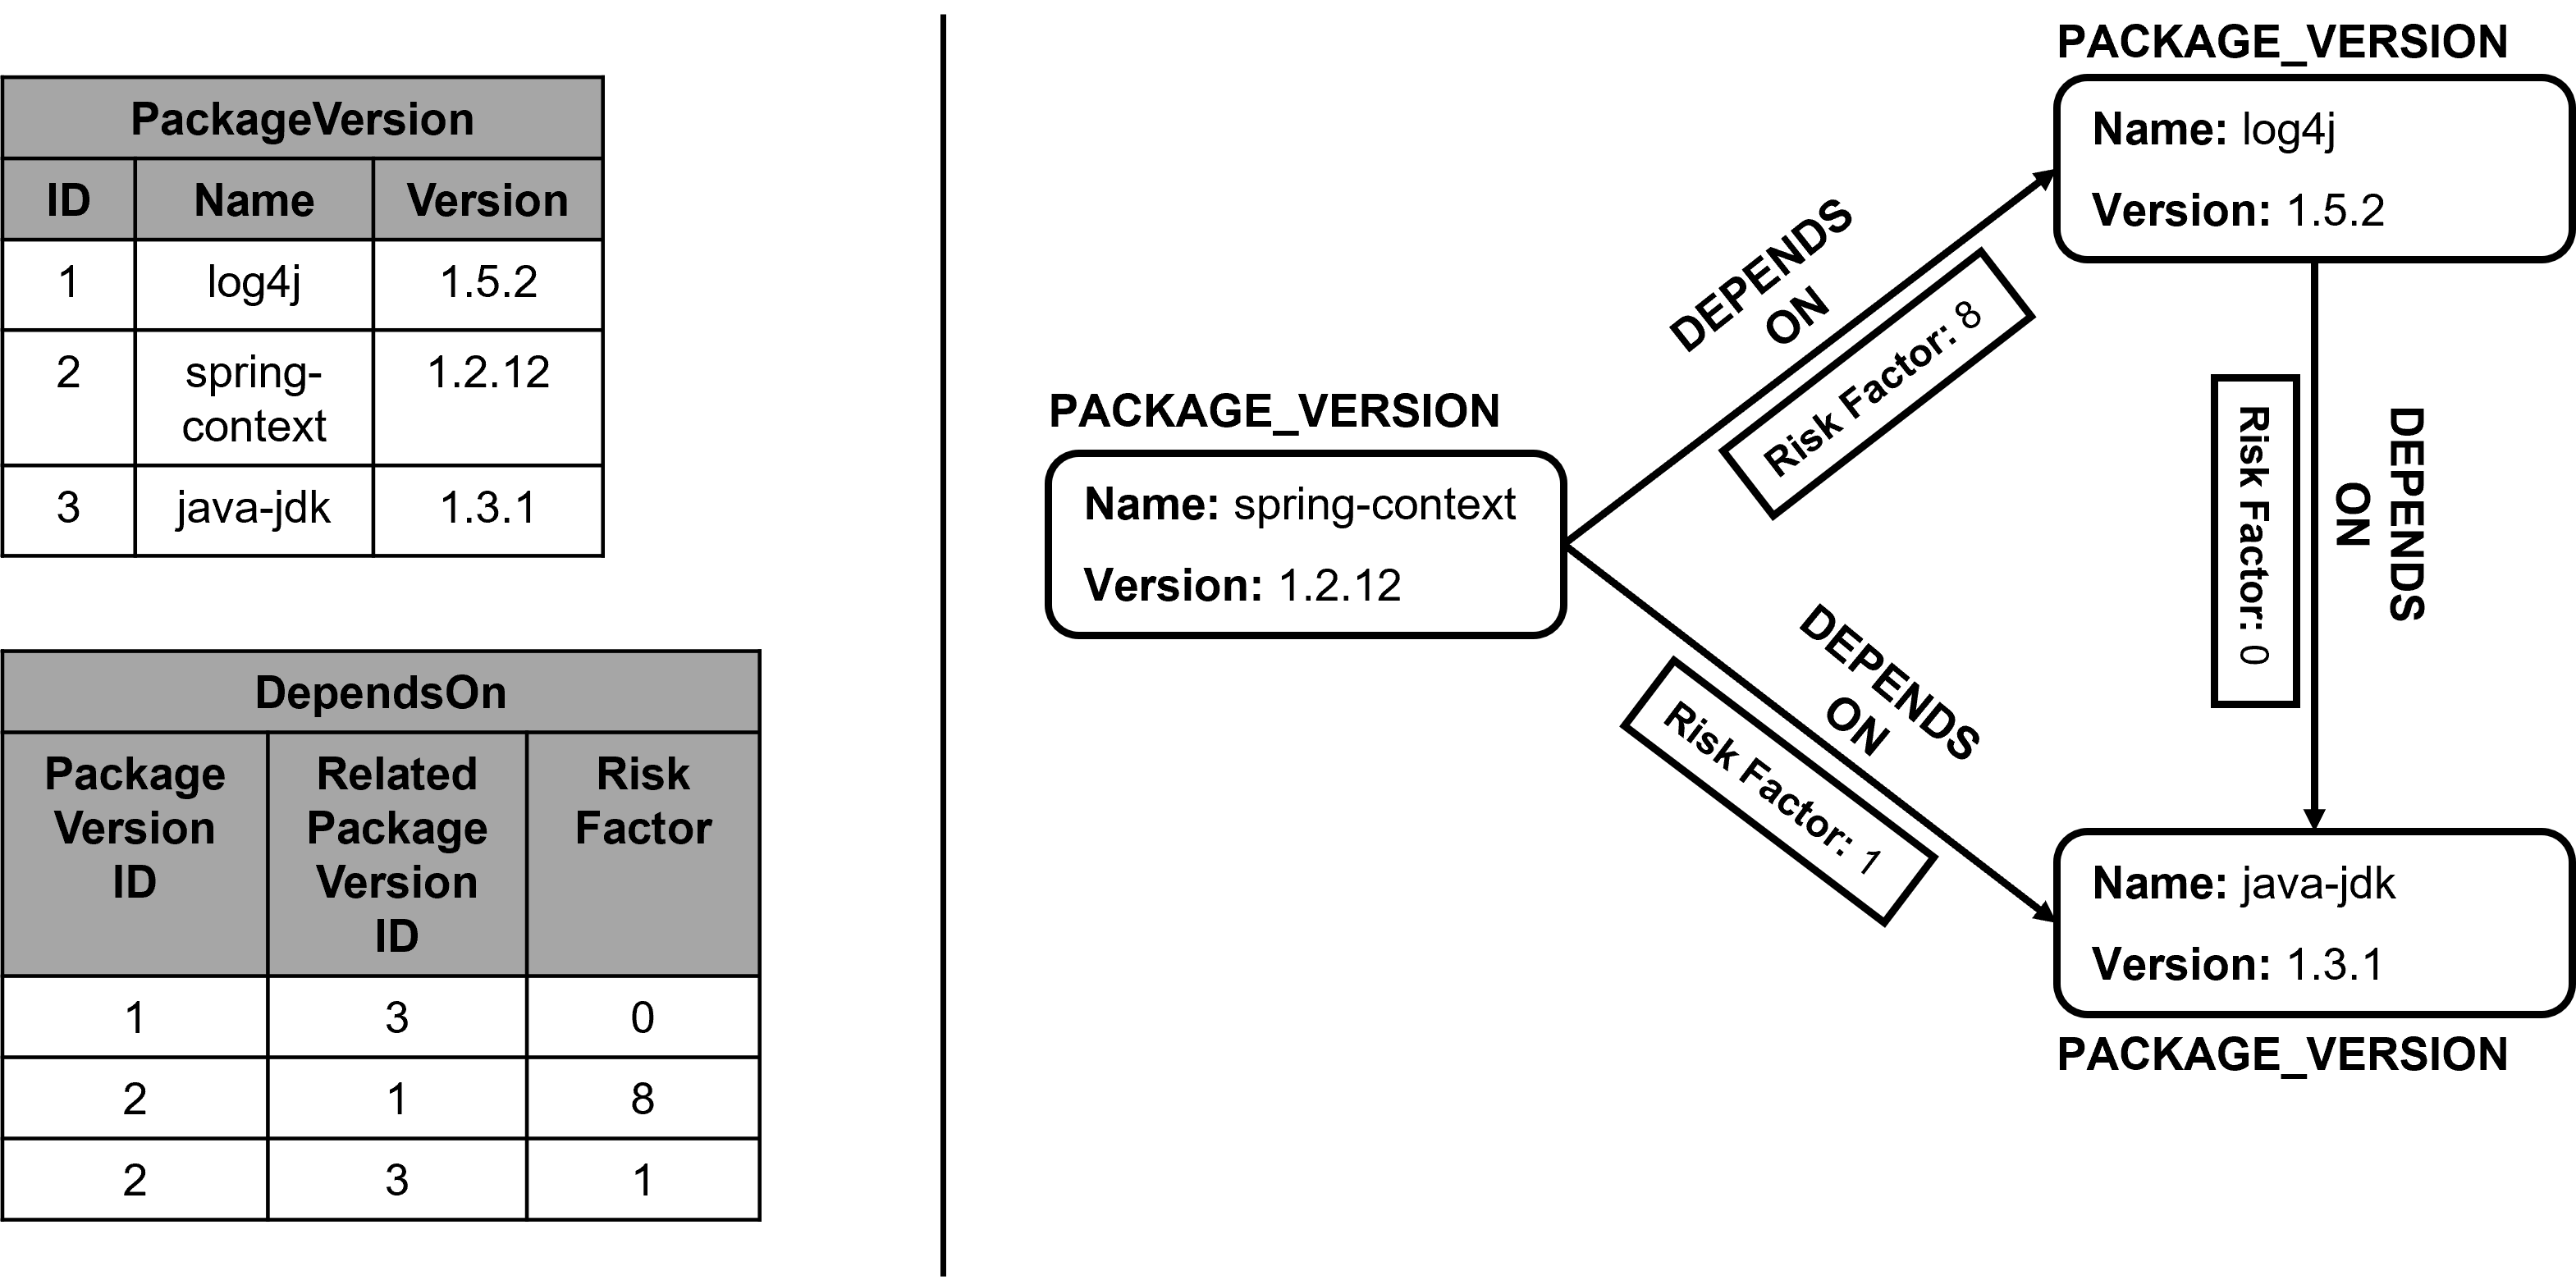
\includegraphics[scale=0.60]{graphdb}
	\caption[Graph Database Representation]{Graph Database Representation}
	\label{fig:GraphDBExample}
\end{figure}

This graph model is called \emph{labeled property graph}. As defined in the "Graph Databases - New Opportunities for Connected Data" written by engineers of the Neo4j database, a labeled property graph has the following characteristics \cite{neo4j}:

\begin{quote}
	\begin{enumerate}
		\item\textit{It contains nodes and relationships. }
		\item\textit{Nodes contain properties (key-value-pairs). }
		\item\textit{Nodes can be labeled with one or more labels. }
		\item\textit{Relationships are named and directed, and always have a start and end node. }
		\item\textit{Relationships can also contain properties. }
	\end{enumerate}
\end{quote}

This model is generally quite intuitive. But obviously, even in this more complex example, with the suitable interpretation of the table (thus, instead of interpreting the relation itself, the foreign key relationships are considered), it still expresses the same graph as the nodes and relationships. And, as discussed previously, document databases are able to express this graph as well, either also through a normalized model or through nested documents.\\\\ 
\emph{So the key difference of graph databases is not that they store graphs in general. The key difference is that their file organization and data processing is optimized to work with graph data.}\par
As shown in figure \ref{fig:GraphDBExample} on the left bottom, table representations and consequently relational databases use an index to link entities, or in this context rather nodes. To increase the performance of reciprocal queries, an additional index may be created on \emph{Related Package Version ID}. These \emph{indexes are global}, so as the graph grows, so do the indexes.\par 
In contrast, in graph databases with native processing capabilities each node often maintains direct references to link nodes. Thus, each node maintains kind of a \emph{local index} whose size and consequently performance do not depend on the total size of the graph. This concept of linking adjacent nodes is commonly referred to as \emph{index-free adjacency}.\footnote{There has been a lot of discussion whether index-free adjacency is a requirement for graph databases \cite{graphdbdiscussion}. The current consensus seems to be that it is not, since especially ArangoDB developed another approach to the problem which allows similar complexities as index-free adjacency for traversing graphs \cite{arangodbhybridindexes}.} For further assumptions and explanations, the architecture of the Neo4j database is considered \cite{neo4j}.\par
So, when querying "Which Package Versions does the spring-context:1.2.12 Package Version depend on?", the initial look up still has a complexity of $O(log(n))$, but finding the related packages is $O(1)$ instead of $O(log(n))$. Since nodes maintain references to nodes with incoming as well as to nodes with outgoing relationships, the reciprocal query "Which Package Versions depend on the spring-context:1.2.12 Package Version?" may be answered with the exact same complexity \cite{neo4j}.\par 
So given this complexities, in theory graph databases scale and perform better than other database technologies when the application involves a lot of graph traversals.\footnote{As before, this theoretical foundation chapter is obviously not complete. Especially the file organization which enables the fast traversals are an interesting topic. For a good and thorough explanation of a implementation, refer to "Graph Databases - New Opportunities for Connected Data" \cite{neo4j}.}

\subsubsection{Suitability for the Central Metadata Store}
This suitability section takes a similar approach as the first one evaluating the suitability of the relational database. Thus, examining the same representative \emph{Package Version} example. This allows for a direct comparison afterwards. Below figure \ref{fig:PackageVersionsAndDependenciesGraph} therefore illustrates the equivalent example from \ref{sec:Theoretical Foundations Relational Database} "Theoretical Foundations" of relational databases as a classical graph.

\begin{figure}[H]
	\centering
	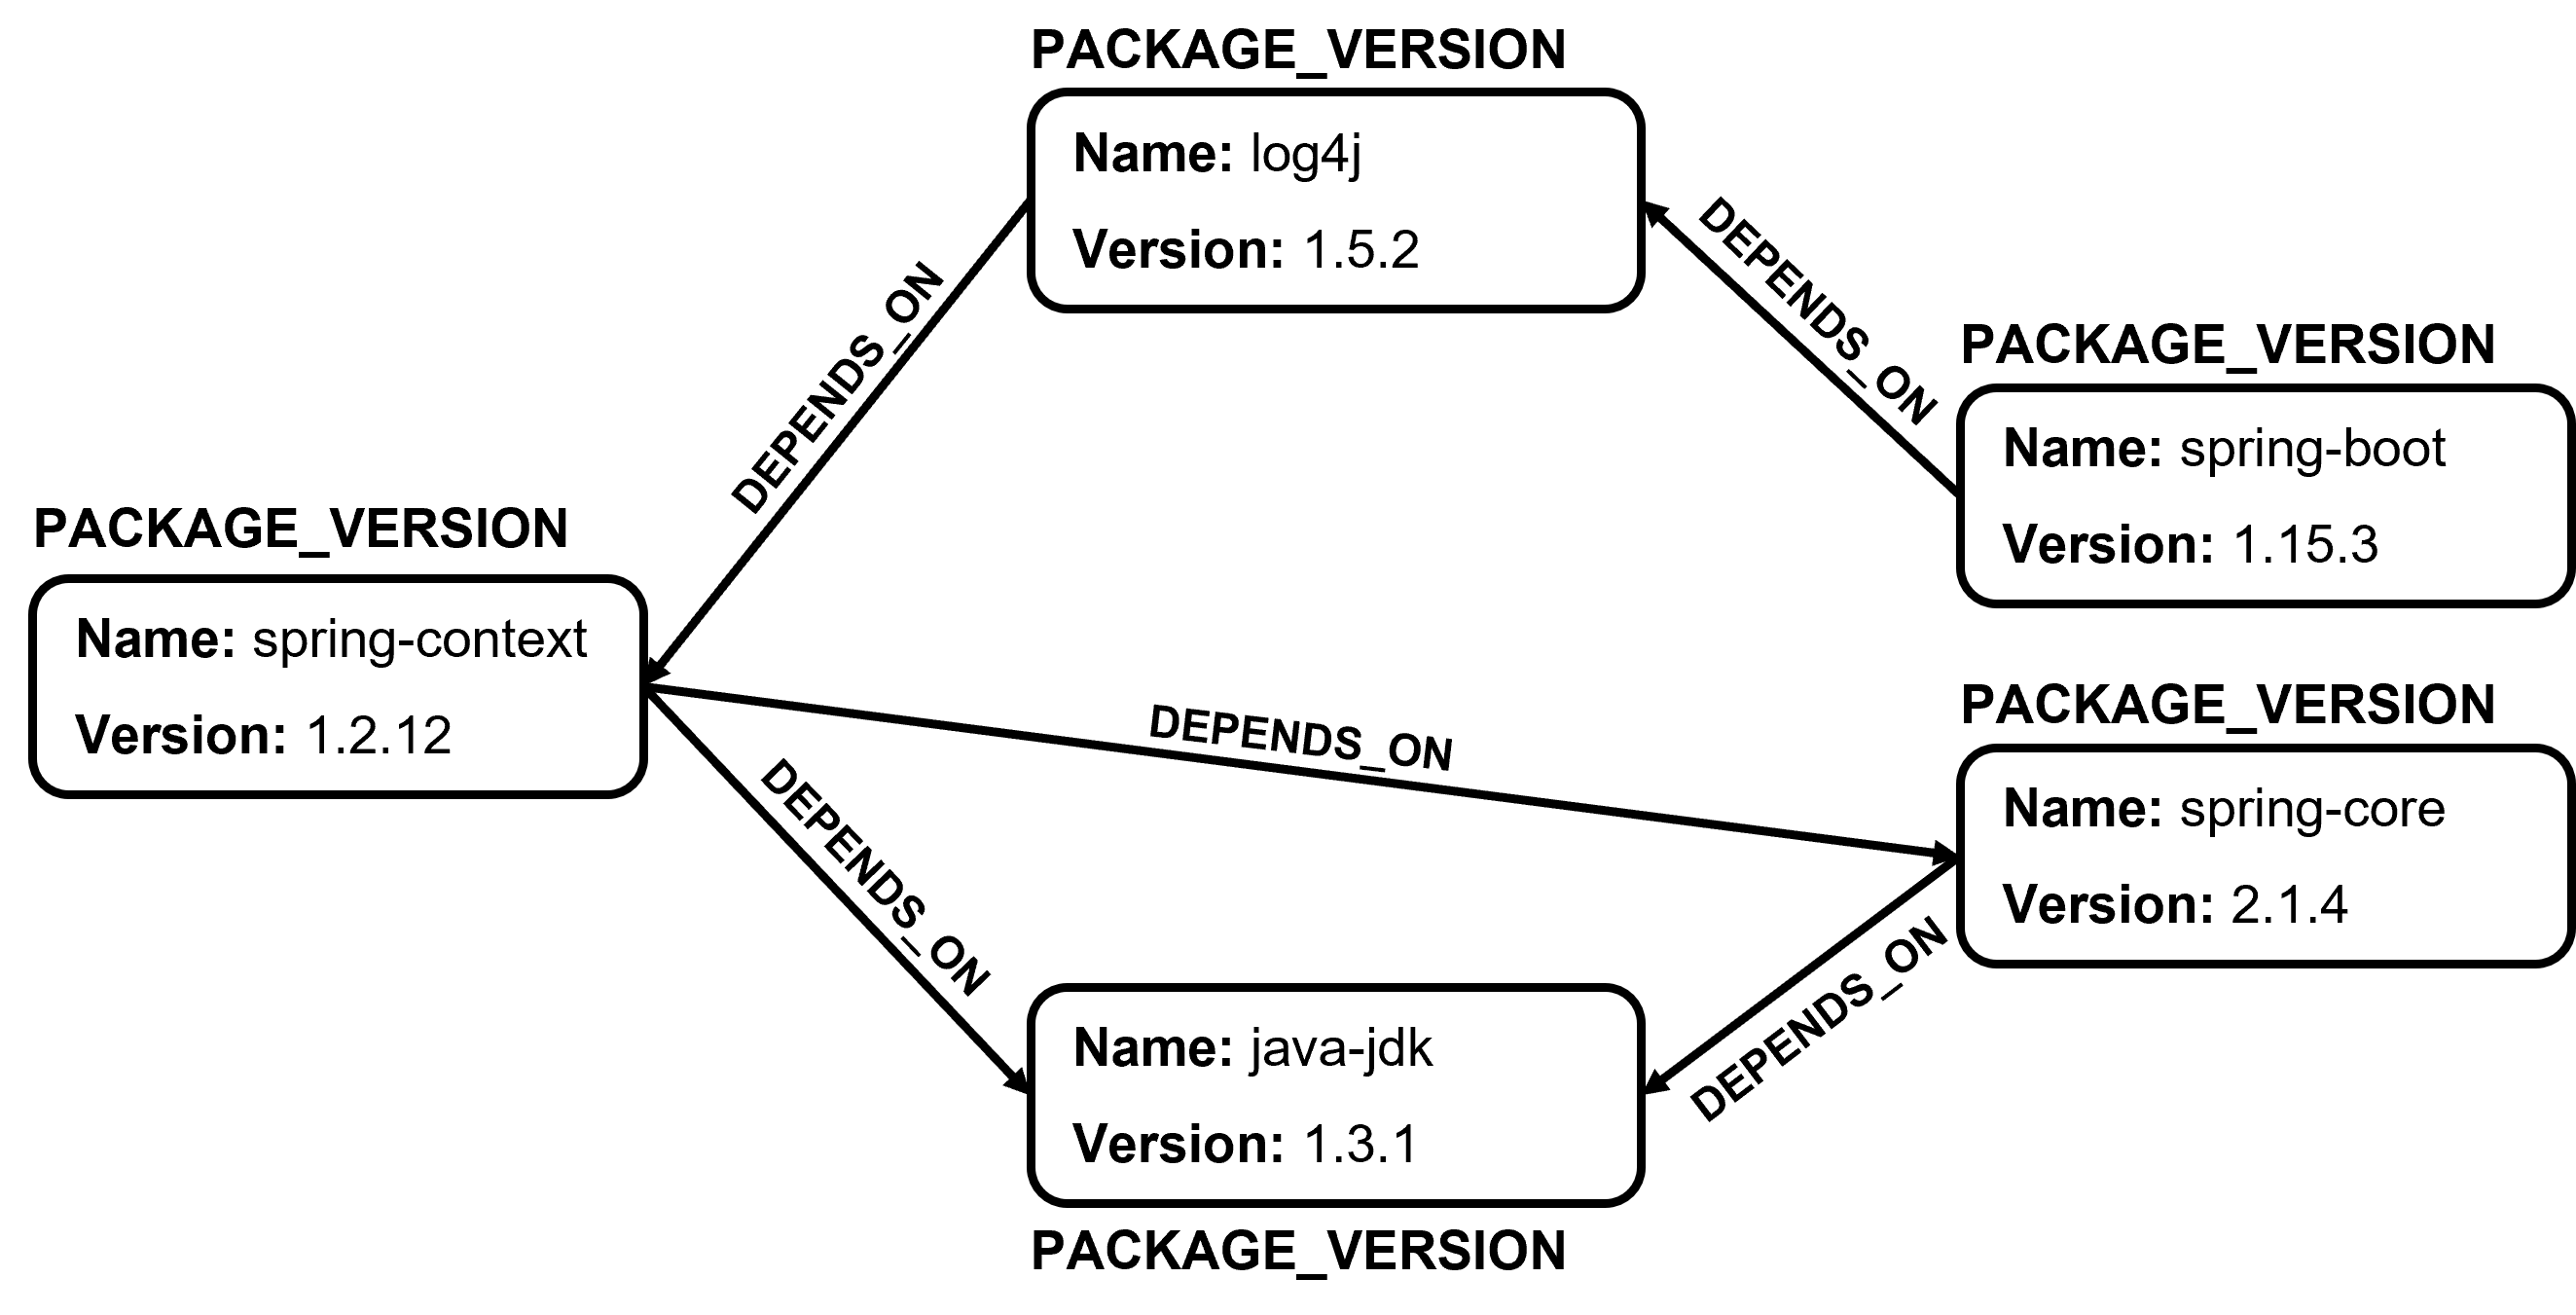
\includegraphics[scale=0.60]{dependency_graph}
	\caption[Package Versions and Dependencies as Graph]{Package Versions and Dependencies as Graph}
	\label{fig:PackageVersionsAndDependenciesGraph}
\end{figure}

Neo4j defines its own SQL inspired language called \emph{cypher}. To answer the respective question "Which Package Version does the spring-context:1.2.12 Package Version depend on?" in Neo4j, the following cypher query would have to be used:

\begin{lstlisting}[caption=Package Version Dependencies (including transitive), captionpos=b, label=lst:CypherTransitive]
MATCH (p1:PACKAGE_VERSION {Name:"spring-context",Version:"1.2.12"})
MATCH (p2:PACKAGE_VERSION)
WHERE (p1)-[:DEPENDS_ON*1..]->(p2)
RETURN (p2)
\end{lstlisting}

The first line in listing \ref{lst:CypherTransitive} matches the node with the \emph{label} \lstinline|PACKAGE_VERSION| and the key-value-pairs \lstinline|Name: "spring-context"| and \lstinline|Version: "1.2.12"| and assigns the resulting nodes, or in this example rather node as there is just a single one that fulfills this pattern, to the variable \lstinline|p1|. The second line and third line matches all nodes with the \emph{label} \lstinline|PACKAGE_VERSION| that \lstinline|p1| depends on. Thus, the \lstinline|WHERE| uses a path as a predicate. Thereby, \lstinline|DEPENDS_ON| specifies the \emph{label} of the relationship and the part after the asterisk specifies the minimum and maximum amounts of hops between the nodes. In this case, the minimum is 1 because otherwise it would consider itself and as there is no explicit maximum given, it defaults to infinite, to consider all transitive dependencies. The nodes that fulfill this criteria are assigned to \lstinline|p2| and returned. In this case, \emph{java-jdk 1.3.1} and \emph{spring-core 2.1.4}.\par 
Assuming there is a composite index on \emph{Name} and \emph{Version}, the initial look up of the node has a time complexity of $O(log(n))$ with $n$ being the number of all nodes with the label \emph{PACKAGE\_VERSION} \cite{neo4j}. The consecutive look ups then have a time complexity of $O(m)$ with $m$ being the number of nodes found during the previous look up. Thus, depending on the number of hops, the general time complexity for such a relationship traversal query may be estimated as 
$$O(log(n)) + O(m) + ... + O(m)$$

So theoretically, the graph database performs and scales significantly better than the relational database for this kind of queries. Besides, the query is definitely simpler to read and understand than the SQL query involving Common Table Expressions. Although, SQL it is arguably still easier to learn the Common Table Expression than learning an entire new query language.\par 
Now just for completion, to answer the reciprocal question "Which Package Versions depend on the spring-context:1.2.12 Package Version?", the following cypher query would have to be used:

\begin{lstlisting}[caption=Package Version Reciprocal Dependencies (including transitive), captionpos=b, label=lst:CypherReciprocalTransitive]
MATCH (p1:PACKAGE_VERSION {Name:"spring-context",Version:"1.2.12"})
MATCH (p2:PACKAGE_VERSION)
WHERE (p1)<-[:DEPENDS_ON*1..]-(p2)
RETURN (p2)
\end{lstlisting}

The only difference in this query is the reversed direction of the relationship in line 3. In this case, it return \emph{log4j 1.5.2} and \emph{spring-boot 1.15.3}. The respective cypher statements to set up the sample data are included in appendix \ref{apx:Data Definition Statement for Neo4J Sample Data}.\par
Besides the efficient traversal of relationship with rather simple queries, there are some other aspects to consider with graph databases. Generally, most graph databases support transactions with \emph{ACID compliance} \cite{neo4jtransactions, arangodbtransactions}. Also, there are some mechanisms to support \emph{referential integrity}, but those do not work exactly as in relational databases. So, in graph databases there is no way to create a relationship to or from a node that does not exist. Furthermore, nodes cannot be deleted as long as relationships to or from that node exist. But compared to relational databases, there is no option to cascade a delete \cite{neo4jdelete}.\par
Regarding \emph{schemas}, or the general storage model, different graph databases vary. Neo4j, for example, only supports key-value properties on nodes or relationships. This is considered as single model graph database. In contrast, in ArangoDB every node is a JSON document, which is considered as multi model graph database \cite{arangodbdocuments}. Therefore, Neo4j does not really have a classical schema. But is still offers several types of constraints such as \emph{unique node property constraints}, \emph{node property existence constraints} and \emph{relationship property existence constraints} to enforce a specific data model \cite{neo4jconstraints}. Similar to MongoDB, for ArangoDB a schema may be enforced on application level \cite{arangodbschema}.

\subsection{Database Selection}
So, a conclusion of the this analysis of the suitability of database technologies for a central metadata store.\par 
\emph{Relational databases} are a solid choice. As shown in the corresponding suitability section, modern SQL provides all features necessary to conveniently implement the required functionality. But the computational complexity of joins is 
$$O(log(n)) + O(m*log(n)) + ... + O(m*log(n))$$
As traversing relationships is involved in the prospectively most frequently used queries, this is a quite important measure.\par 
\emph{Document databases} are not the technology for this application. As it does not allow for significant de-normalization since the access patterns are versatile, the document database does not have an advantage over a relational database.\par 
\emph{Graph databases} are optimized for relationship traversal. The previous section has also shown that the cypher queries are simple in comparison to SQL. Due to its purpose, its computational complexity of traversing relationships is better than with relational databases
$$O(log(n)) + O(m) + ... + O(m)$$
So, the graph database seems to be the theoretically best database technology for this application. In practice, it also has to be considered, that the application has to be supported and there is less experience around graph databases. This also increases the chances of unforeseen queries or other situation, where the graph database may be a problem.\par 
For the scope of this work, the graph database is chosen for the implementation to further evaluate its suitability and practicality.\\\\
The concrete graph database solutions considered were primarily Neo4j and ArangoDB. Neo4j because it has an open source community edition, good documentation and a supportive community. ArangoDB mainly because it is multi model and therefore enables storing JSON, which offers greater flexibility.\par 
Finally, Neo4j was chosen as it seemed to be the better fit over all. Even in the situations where JSON has to be stored, it is rarely necessary to traverse into the document structure. So it is usually sufficient to access the JSON document by its key which may also be done in Neo4j.  












 
 


\section{API}

